\documentclass[a4paper, 12pt]{article}
\usepackage{lmodern}
\usepackage{amssymb,amsmath}
\usepackage{ifxetex,ifluatex}
\usepackage{fixltx2e} % provides \textsubscript
\ifnum 0\ifxetex 1\fi\ifluatex 1\fi=0 % if pdftex
  \usepackage[T1]{fontenc}
  \usepackage[utf8]{inputenc}
\else % if luatex or xelatex
  \ifxetex
    \usepackage{mathspec}
  \else
    \usepackage{fontspec}
  \fi
  \defaultfontfeatures{Ligatures=TeX,Scale=MatchLowercase}
\fi
% use upquote if available, for straight quotes in verbatim environments
\IfFileExists{upquote.sty}{\usepackage{upquote}}{}
% use microtype if available
\IfFileExists{microtype.sty}{%
\usepackage{microtype}
\UseMicrotypeSet[protrusion]{basicmath} % disable protrusion for tt fonts
}{}
\usepackage[left=3.5cm,right=2.5cm,top=2.5cm,bottom=2.5cm]{geometry}
\usepackage{hyperref}
\PassOptionsToPackage{usenames,dvipsnames}{color} % color is loaded by hyperref
\hypersetup{unicode=true,
            pdftitle={Regressão Quantílica},
            pdfauthor={Luiz Fernando Palin Droubi; Carlos Augusto Zilli; Murilo Damian Ribeiro; Norberto Hochheim},
            colorlinks=true,
            linkcolor=red,
            citecolor=green,
            urlcolor=magenta,
            breaklinks=true}
\urlstyle{same}  % don't use monospace font for urls
\usepackage{graphicx,grffile}
\makeatletter
\def\maxwidth{\ifdim\Gin@nat@width>\linewidth\linewidth\else\Gin@nat@width\fi}
\def\maxheight{\ifdim\Gin@nat@height>\textheight\textheight\else\Gin@nat@height\fi}
\makeatother
% Scale images if necessary, so that they will not overflow the page
% margins by default, and it is still possible to overwrite the defaults
% using explicit options in \includegraphics[width, height, ...]{}
\setkeys{Gin}{width=\maxwidth,height=\maxheight,keepaspectratio}
\IfFileExists{parskip.sty}{%
\usepackage{parskip}
}{% else
\setlength{\parindent}{0pt}
\setlength{\parskip}{6pt plus 2pt minus 1pt}
}
\setlength{\emergencystretch}{3em}  % prevent overfull lines
\providecommand{\tightlist}{%
  \setlength{\itemsep}{0pt}\setlength{\parskip}{0pt}}
\setcounter{secnumdepth}{5}
% Redefines (sub)paragraphs to behave more like sections
\ifx\paragraph\undefined\else
\let\oldparagraph\paragraph
\renewcommand{\paragraph}[1]{\oldparagraph{#1}\mbox{}}
\fi
\ifx\subparagraph\undefined\else
\let\oldsubparagraph\subparagraph
\renewcommand{\subparagraph}[1]{\oldsubparagraph{#1}\mbox{}}
\fi

%%% Use protect on footnotes to avoid problems with footnotes in titles
\let\rmarkdownfootnote\footnote%
\def\footnote{\protect\rmarkdownfootnote}

%%% Change title format to be more compact
\usepackage{titling}

% Create subtitle command for use in maketitle
\providecommand{\subtitle}[1]{
  \posttitle{
    \begin{center}\large#1\end{center}
    }
}

\setlength{\droptitle}{-2em}

  \title{Regressão Quantílica}
    \pretitle{\vspace{\droptitle}\centering\huge}
  \posttitle{\par}
  \subtitle{Aplicações na Engenharia de Avaliações}
  \author{Luiz Fernando Palin Droubi\footnote{SPU/SC,
  \href{mailto:lfpdroubi@gmail.com}{\nolinkurl{lfpdroubi@gmail.com}}} \\ Carlos Augusto Zilli\footnote{IFSC,
  \href{mailto:carloszilli@gmail.com}{\nolinkurl{carloszilli@gmail.com}}} \\ Murilo Damian Ribeiro\footnote{UFSC,
  \href{mailto:murilodamianr@gmail.com}{\nolinkurl{murilodamianr@gmail.com}}
} \\ Norberto Hochheim\footnote{UFSC,
  \href{mailto:hochheim@gmail.com}{\nolinkurl{hochheim@gmail.com}}}}
    \preauthor{\centering\large\emph}
  \postauthor{\par}
      \predate{\centering\large\emph}
  \postdate{\par}
    \date{05/11/2019}

\usepackage[brazil]{babel}
\usepackage{graphicx}
\usepackage{float}
\usepackage{subfig}
\usepackage{caption}
\usepackage{lastpage}
\setlength{\parindent}{1.25cm} % Default is 15pt.
\usepackage{indentfirst}
\usepackage{fontspec} % para Arial
\setmainfont{Arial}
\newcommand{\pkg}[1]{{\normalfont\fontseries{b}\selectfont #1}}
\let\proglang=\textsf
\let\code=\texttt
\newcommand{\bcenter}{\begin{center}}
\newcommand{\ecenter}{\end{center}}
\usepackage{fancyhdr}
% Turn on the style
\pagestyle{fancy}
% Clear the header and footer
\fancyhead{}
\fancyfoot{}
% Set the right side of the footer to be the page number
\fancyfoot[R]{\thepage~/~\pageref{LastPage}}

\begin{document}
\maketitle

\hypertarget{introducao}{%
\section{Introdução}\label{introducao}}

Segundo Koenker (\protect\hyperlink{ref-mim}{2009}, p. 371), o gráfico
mais importante da história da estatística é o gráfico de Galton, por
nós reproduzido na figura \ref{fig:galton}.

O gráfico ilustra o fenômeno, descoberto por Galton, da regressão à
média.

\begin{figure}
\centering
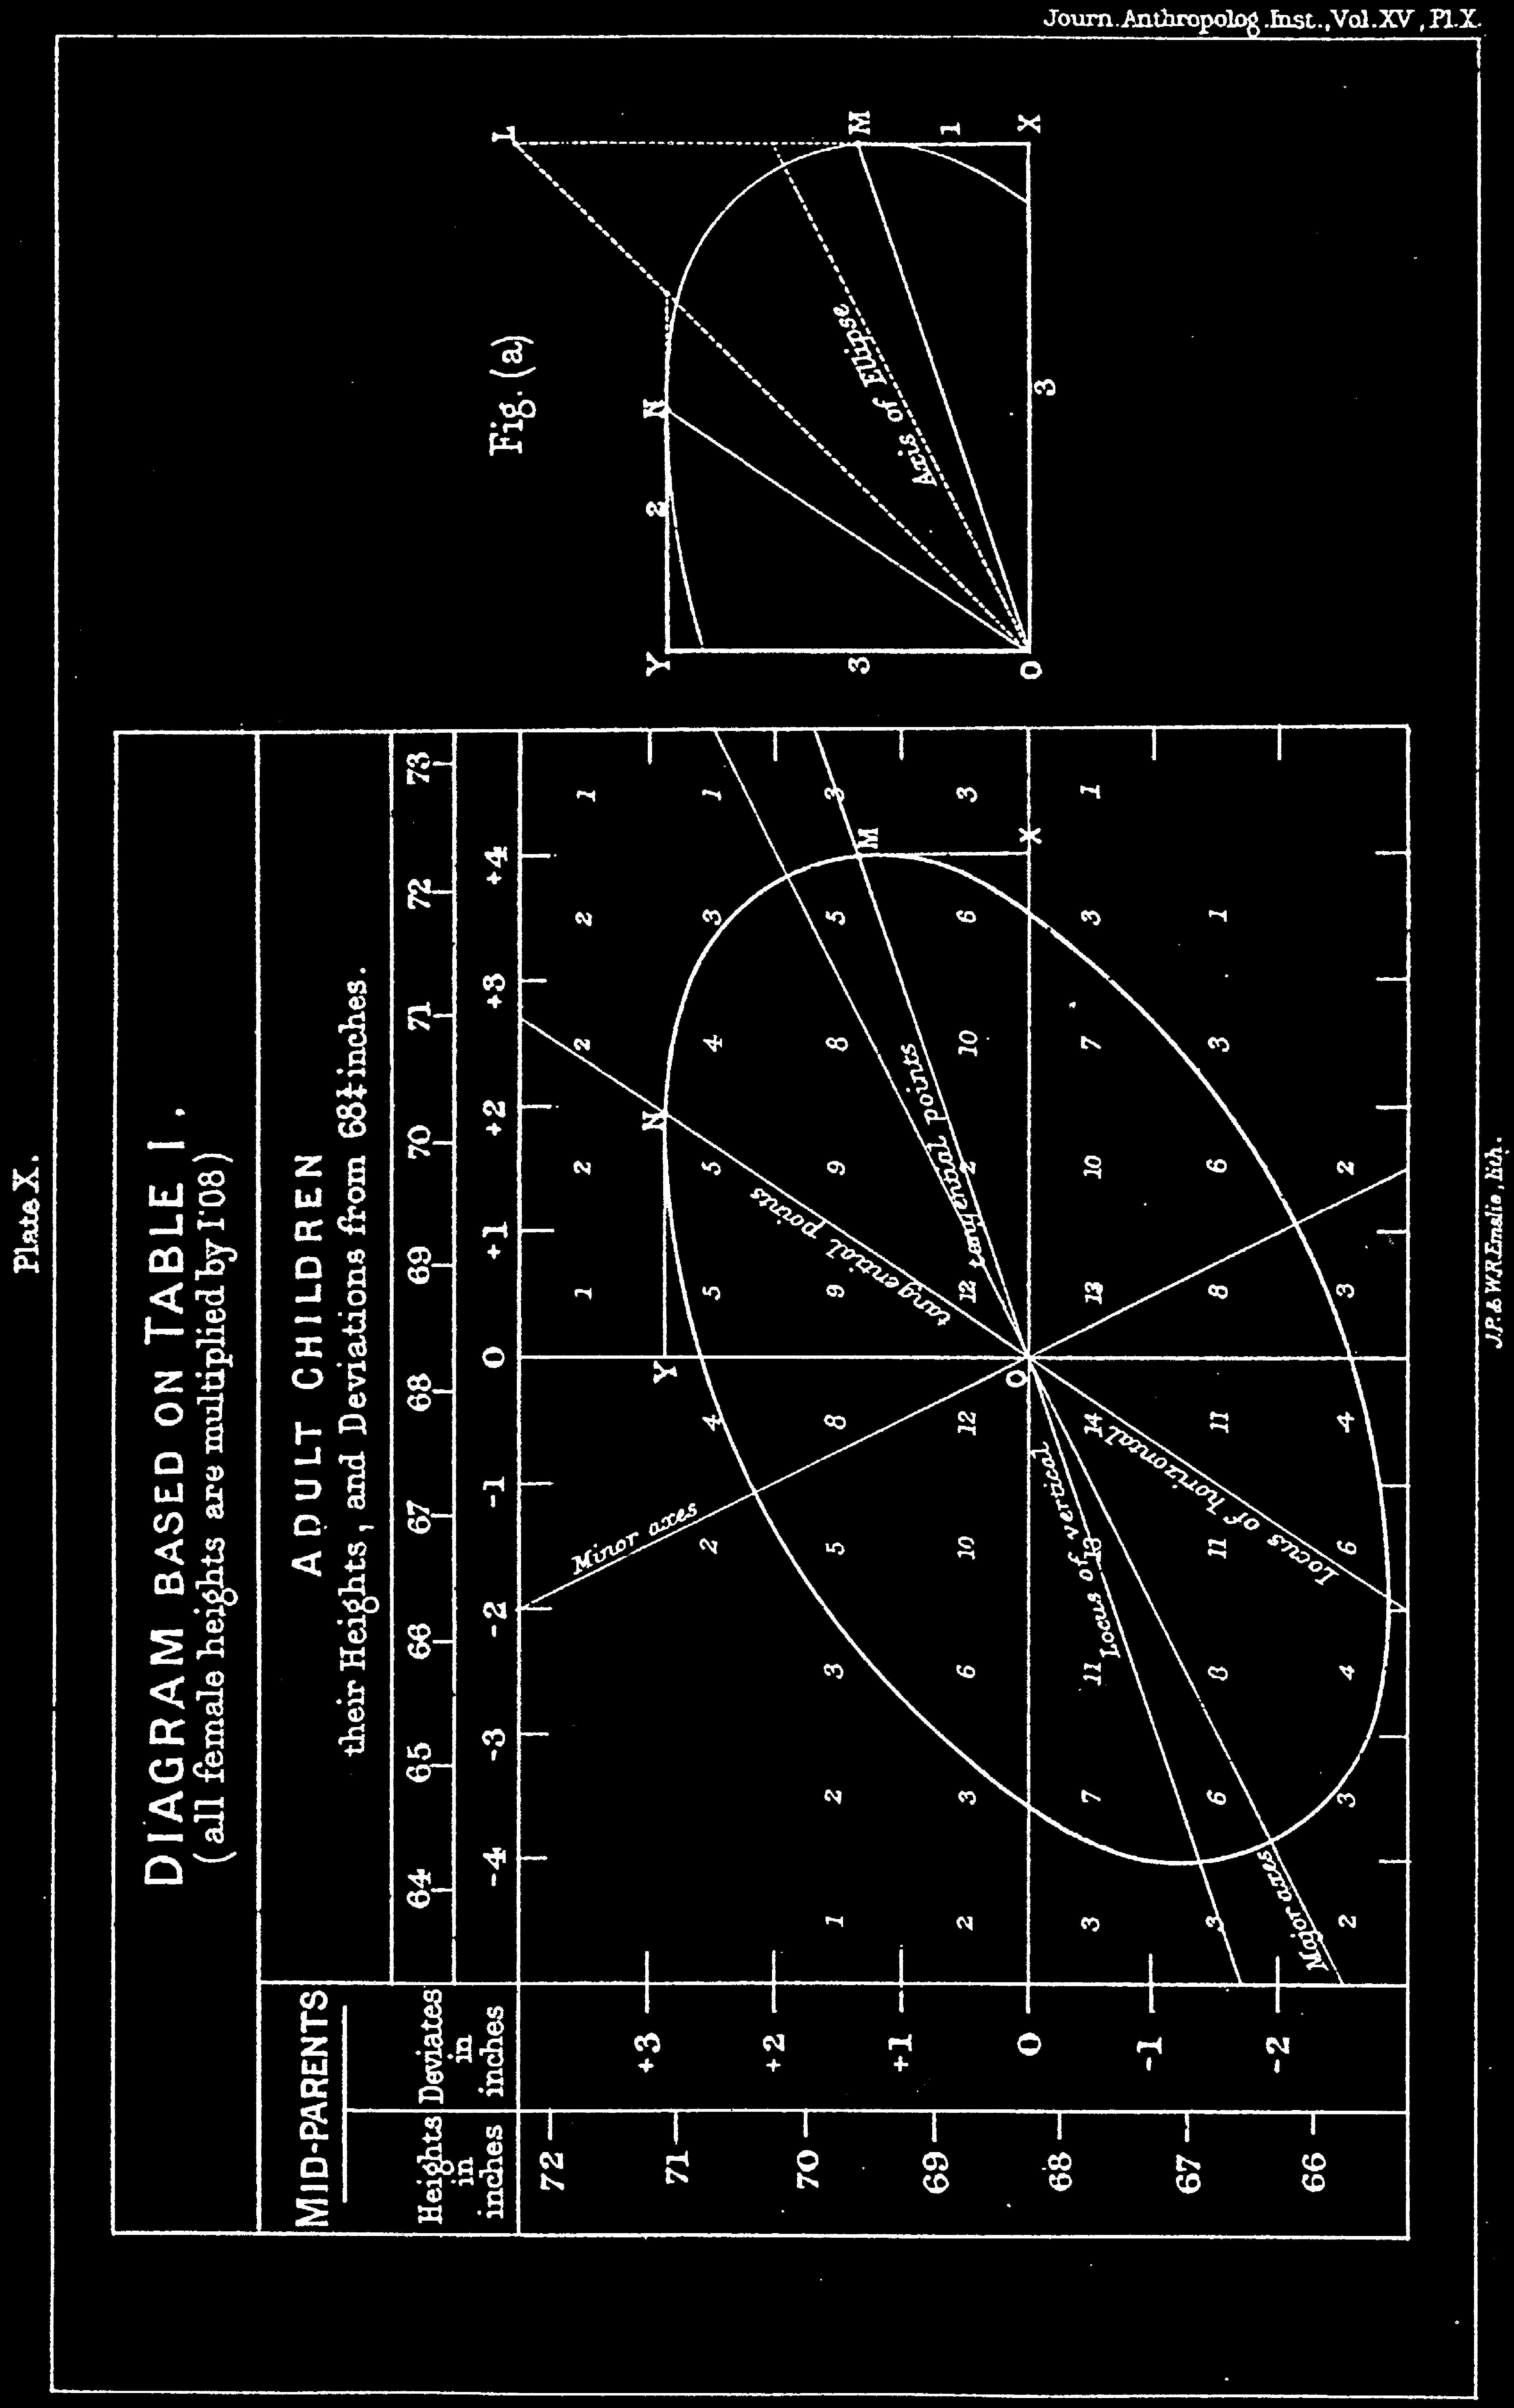
\includegraphics{refs/image-002.png}
\caption{Regressão à média (Galton, 1885)}
\end{figure}

\hypertarget{breve-historico}{%
\section{Breve Histórico}\label{breve-historico}}

Boscovich propôs em 1760 (PORTNOY; KOENKER,
\protect\hyperlink{ref-tortoise}{1997}, p. 281) -- portanto ainda antes
da introdução do método dos mínimos quadrados por Legendre em
1805\footnote{Gauss ligou o método dos mínimos quadrados à distribuição
  normal em seu trabalho intitulado \emph{Theoria Motus Corporum
  Coelestium} de 1809 mas a origem do método se deve ao trabalho
  pioneiro de Legendre. Houve discordâncias entre os dois na disputa
  pela invenção do método, e outros achados na época. Ver a este
  respeito STIGLER (\protect\hyperlink{ref-STIGLER197731}{1977}).}, no
seu trabalho intitulado \emph{Nouvelles méthodes pour la determination
des orbites des comètes} --, o seguinte problema:

Encontrar \(\hat \alpha\) e \(\hat \beta\) tais que:

\[y_i = \hat \alpha + \hat \beta x_i + \hat u_i\]

com \(\sum \hat u_i = 0\) e \(\sum |\hat u_i| = \text{min!}\).

Laplace resolveu o problema matematicamente em 1789 (PORTNOY; KOENKER,
\protect\hyperlink{ref-tortoise}{1997}, p. 281).

Posteriormente, com a chegada do \emph{méthode de moindre carré}, ou
seja, do método dos mínimos quadrados ordinários, o método dos mínimos
erros absolutos de Laplace ficou em segundo plano, até que Edgeworth, em
1887 propõe o primeiro algoritmo capaz de obter o intercepto e o
coeficiente angular da reta do método dos mínimos desvios absolutos,
relaxando a restrição de que a soma dos resíduos seja igual a zero
(\(\sum \hat u_i = 0\)) (PORTNOY; KOENKER,
\protect\hyperlink{ref-tortoise}{1997}, p. 281).

Na década de 40 surgiram os primeiros algoritmos simplex destinados à
otimização, algoritmos estes que se ajustam às necessidades do métodos
dos mínimos desvios absolutos, que não possui solução analítica, mas
iterativa. A primeira aplicação do método dos mínimos desvios absolutos
se deve a Arrow e Hoffenberg, em 1959.(PORTNOY; KOENKER,
\protect\hyperlink{ref-tortoise}{1997}, p. 281).

Koenker e Basset (\protect\hyperlink{ref-koenker1978}{1978})
generalizaram o problema de minimização do erro médio absoluto, o que
equivale à regressão à mediana, ao problema de encontrar os diversos
quantis de distribuição através da aplicação de uma função de perda
assimétrica, correspondente àquele quantil, chegando-se assim à
regressão quantílica.

\hypertarget{referencial-teorico}{%
\section{Referencial teórico}\label{referencial-teorico}}

\hypertarget{estimacao-de-quantis}{%
\subsection{Estimação de quantis}\label{estimacao-de-quantis}}

Existem diversas formas de se obter os quantis de uma amostra.

\hypertarget{o-problema-de-estimar-quantis-como-um-problema-de-minimizacao}{%
\subsection{O problema de estimar quantis como um problema de
minimização}\label{o-problema-de-estimar-quantis-como-um-problema-de-minimizacao}}

Pode-se demonstrar que, assim como a média aritmética \(\mu\) de uma
variável aleatória tem a propriedade de minimizar a soma dos desvios
quadráticos de cada observação em relação a ela (MATLOFF,
\protect\hyperlink{ref-matloff2017}{2017}, p. 50), a mediana tem a
propriedade de minimizar a soma dos desvios médios absolutos de cada
observação (MATLOFF, \protect\hyperlink{ref-matloff2017}{2017}, p. 260).
Ou seja:

\[\mu(Y) = \mathbb{E}Y = \arg \min_c \sum_{i = 1}^n \frac{1}{n}(y_i - c)^2\]
\[Me = \arg \min_c \sum_{i = 1}^n \frac{1}{n}|y_i - c|\] Sabe-se que a
mediana de uma variável equivale ao quantil de 50\%. Assim, outros
quantis podem ser obtidos com formulação análoga à formulação acima,
porém com a aplicação de uma função de perda assimétrica
(\(\rho_\tau(.)\)) em lugar da função módulo (ver figura 1):

\[Q_\tau(Y) = \arg \min_c \sum_{i = 1}^n \rho_\tau(y_i - c)\]

\begin{figure}[H]

{\centering 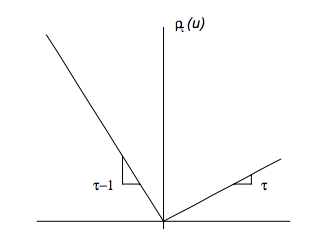
\includegraphics[width=0.7\linewidth]{DmKq7} 

}

\caption{Função de perda ou custo.}\label{fig:unnamed-chunk-1}
\end{figure}

\bcenter Fonte: KOENKER; HALLOCK (\protect\hyperlink{ref-qr}{2001}).
\ecenter

\hypertarget{regressao-linear-e-quantilica}{%
\subsection{Regressão linear e
quantílica}\label{regressao-linear-e-quantilica}}

A regressão linear pode ser vista como uma forma de minimização, assim
como a média de uma população pode ser visto como o problema de
minimização descrito acima.

A diferença é que no caso da regressão linear, ao invés de minimizar em
relação a um escalar, desta vez se minimiza o erro em prever uma
variável Y em relação a {]} uma função de outra variável X, f(X).
Pode-se demonstrar que entre todas as funções f(X), a que minimiza o
erro médio quadrático de Y dado X (\(\mathbb{E}[(Y - f(X))^2]\)) é a
função de regressão \(\mu(t) = \mathbb{E}(Y|X=t)\) (MATLOFF,
\protect\hyperlink{ref-matloff2017}{2017}, pp. 49--50).

Analogamente, pode-se demonstrar que a mediana condicional é a função
que minimiza o erro médio absoluto de Y dado X
(\(\mathbb{E}(|Y-f(X)|)\)) (MATLOFF,
\protect\hyperlink{ref-matloff2017}{2017}, pp. 260--261).

\hypertarget{unicidade-da-solucao}{%
\subsubsection{Unicidade da solução}\label{unicidade-da-solucao}}

Pode-se demonstrar que a regressão linear, ou seja, a minimização de
\(\mathbb{E}[(Y - X\beta)^2]\) possui uma única solução e esta solução
pode ser encontrada analiticamente, bastando para isso efetuar a
derivação parcial deste termo e igualando-o a zero, obtendo-se assum um
único solução para o cálculo do valor de \(\beta\) (ver MATLOFF,
\protect\hyperlink{ref-matloff2017}{2017}, pp. 49--50).

O mesmo não se pode dizer da regressão à mediana a mais genericamente da
regressão quantílica. Nesta abordagem, há múltiplas soluções possíveis,
assim como numa amostra de tamanho par existem duas medianas possíveis.
Ainda, as soluções do problema de minimização da regressão quantílica
não podem ser encontradas analiticamente, sendo necessária a utilização
de precessos iterativos para a obtenção do(s) mínimo(s).

Contudo, deve-se ter em mente que, em ambos os processos de minimização,
seja para a regressão linear ou para a regressão quantílica, trabalha-se
com apenas uma amostra da população estudada. Desta forma, os valores de
\(\hat \beta\) encontrados são apenas estimativas dos valores reais de
\(\beta\), ou seja, os valores da população.

Assim, deve-se levar em conta que a diferença entre as múltiplas
soluções da regressão quantílica é da ordem de \(1/n\), enquanto a
amplitude da precisão da estimativa é de tamanho \(1/\sqrt{n}\). Assim,
presume-se que as múltiplas soluções possíveis, para os casos práticos
estão dentro da margem de erro para a primeira estimativa encontrada
pelo algoritmo.

\hypertarget{robustez-da-solucao}{%
\subsection{Robustez da solução}\label{robustez-da-solucao}}

\hypertarget{transformacao-e-retransformacao}{%
\subsection{Transformação e
retransformação}\label{transformacao-e-retransformacao}}

\[Q_{f(Y)}(\tau) = f(Q_Y(\tau))\]

\hypertarget{eficiencia-computacional}{%
\subsection{Eficiência computacional}\label{eficiencia-computacional}}

\hypertarget{estimador-de-maxima-verossimilhanca}{%
\subsection{Estimador de máxima
verossimilhança}\label{estimador-de-maxima-verossimilhanca}}

Pode-se demonstrar que, quando a distribuição é normal o estimador de
máxima verossimilhança para o parâmetro \(\mu\) da distribuição é a
média amostral.

Analogamente, se a distribuição dos dados for a distribuição de Laplace,
o estimador de máxima verossimilhança para o parâmetro é a mediana.

Isto implica que, se a distribuição dos dados é normal, são necessários
\(\pi/2\) (1,57) vezes mais dados para que a estimativa de \(\mu\)
através da mediana seja tão eficiente quanto a estimativa através da
média. Isto implica, por sua vez, que intervalos de confiança obtidos
para a regressão quantílica são 25\% mais largos do que os intervalos de
confiança para a regressão linear (KOENKER,
\protect\hyperlink{ref-koenker2000}{2000}, p. 354).

No entanto, se a distribuição dos dados for a distribuição de Laplace,
pode-se demonstrar que são necessários duas vezes mais dados para que a
média estime \(\mu\) com a mesma precisão da mediana.

\hypertarget{media}{%
\paragraph{Média}\label{media}}

\begin{figure}[H]

{\centering 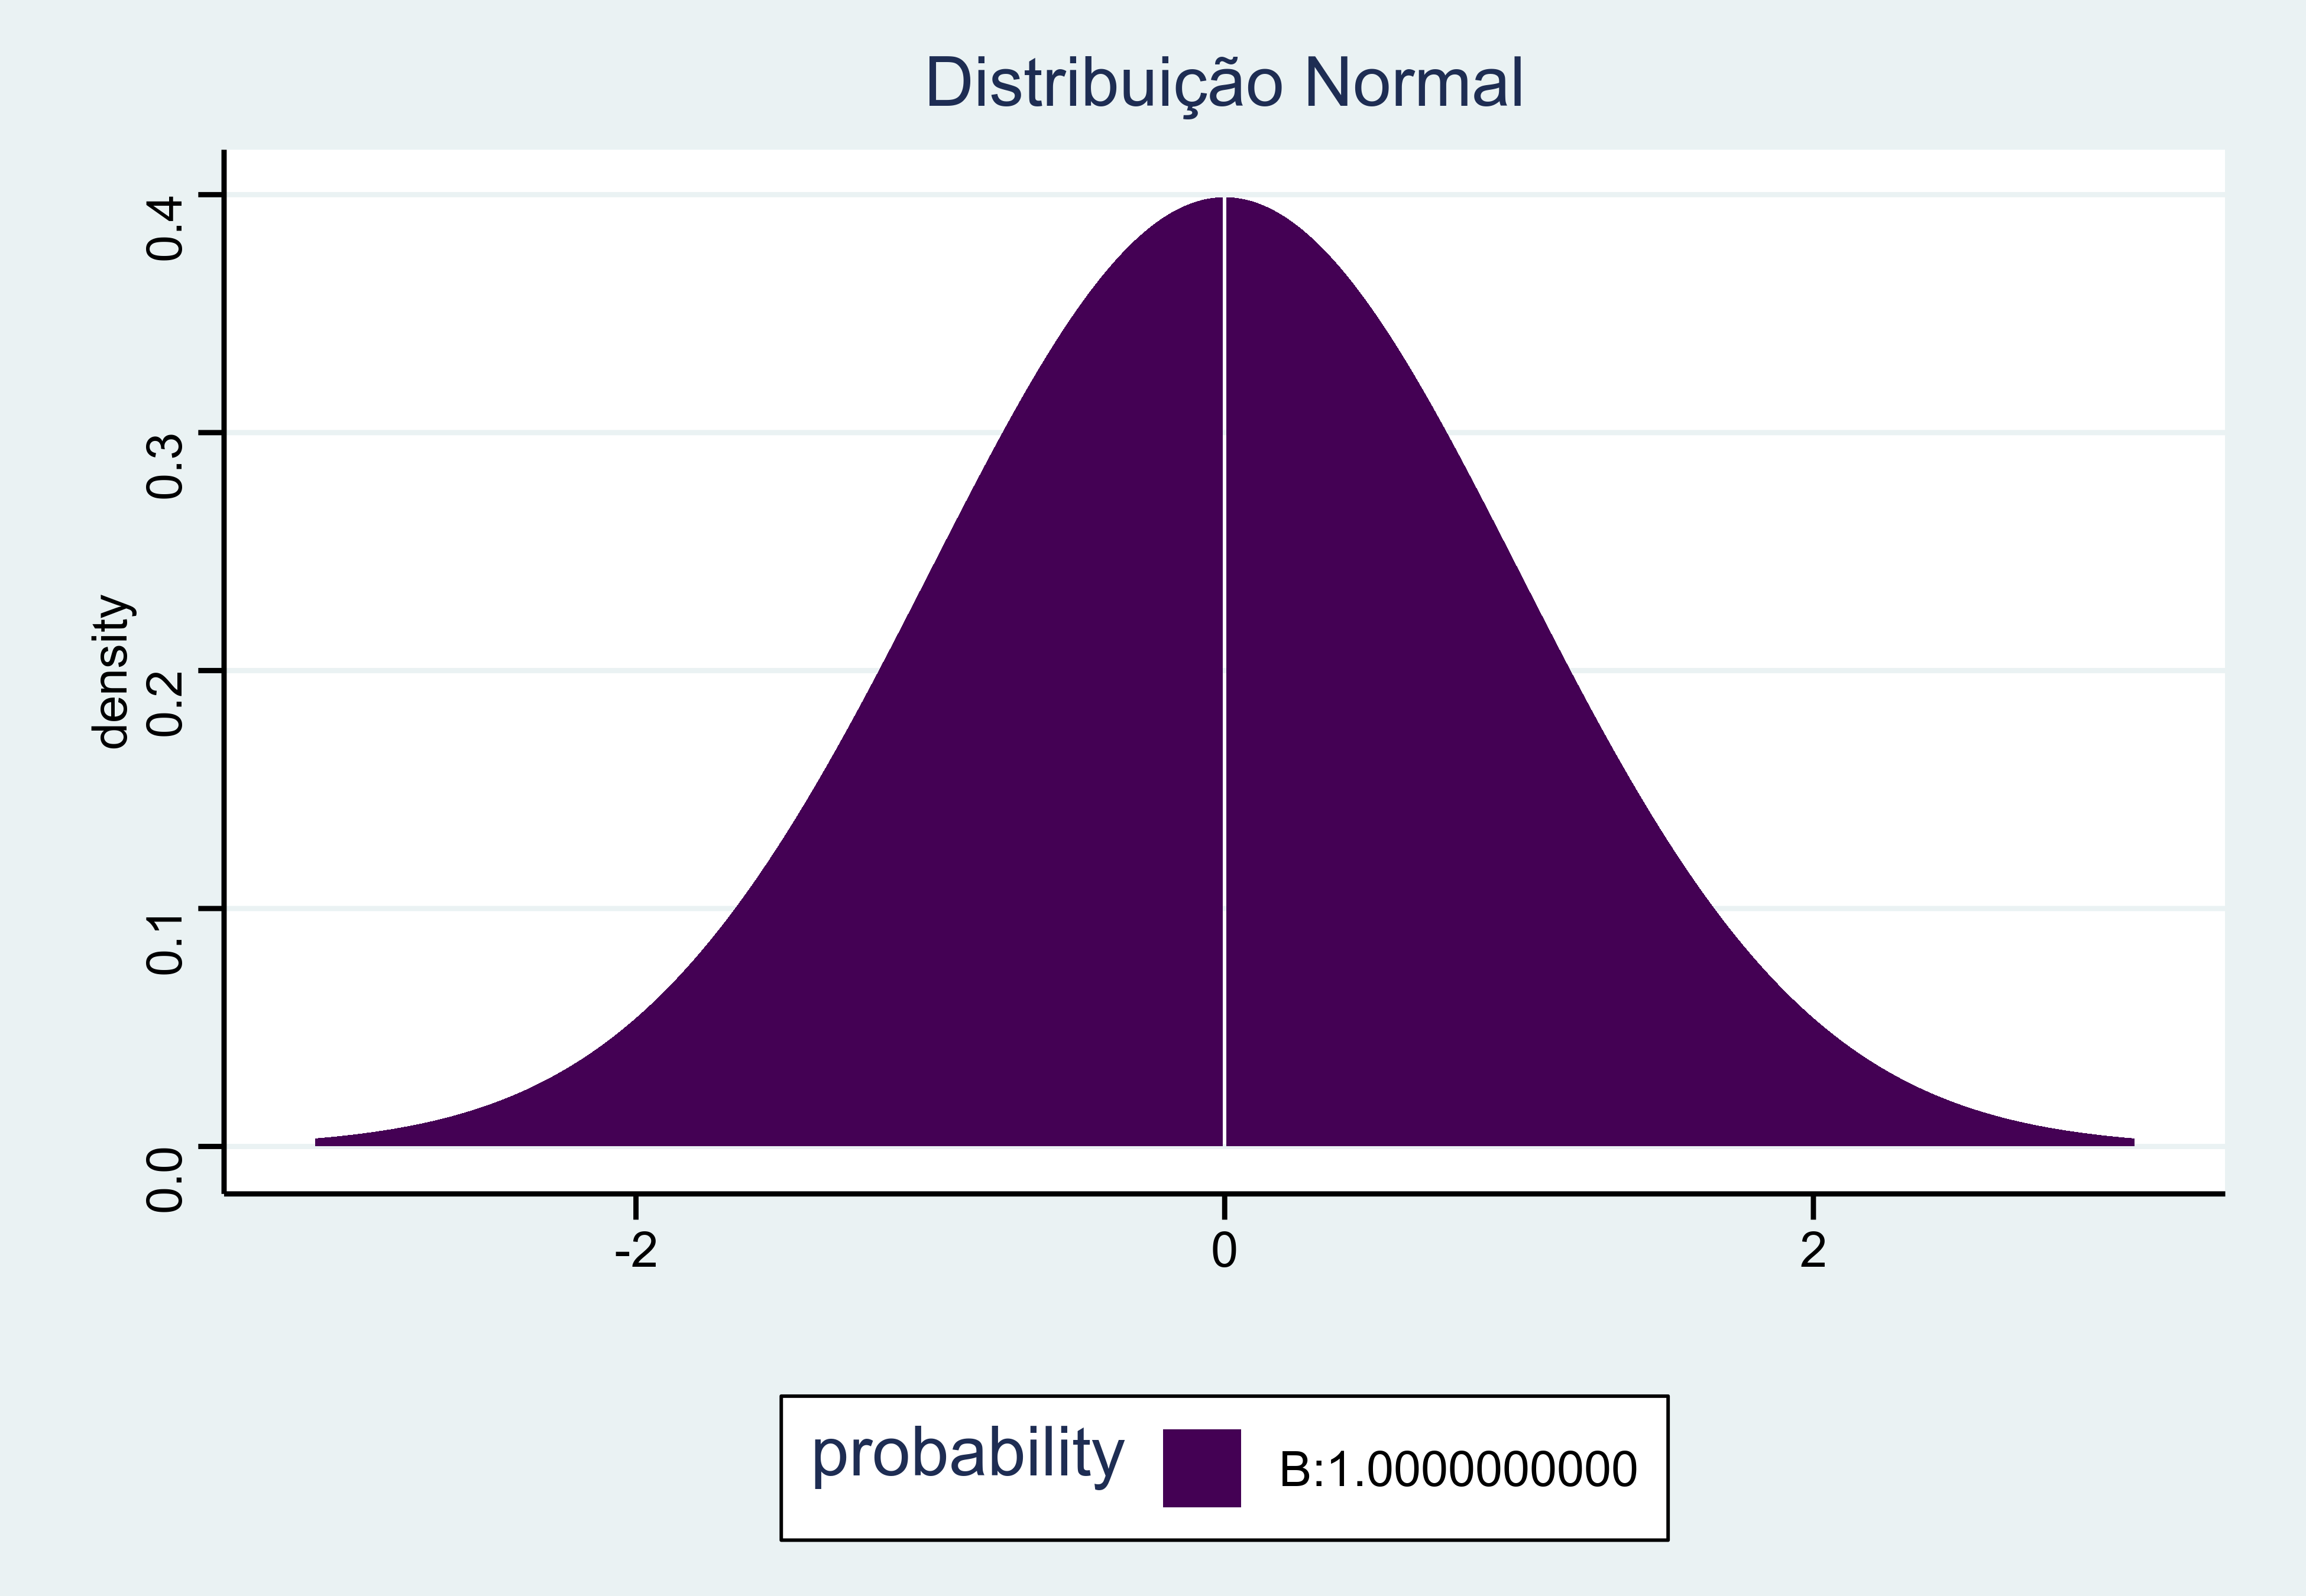
\includegraphics[width=0.7\linewidth]{images/dist_normal-1} 

}

\caption{Distribuição Normal.}\label{fig:dist_normal}
\end{figure}

\[\hat \mu = \frac{1}{n}\sum x_i\]
\[\hat \sigma = \frac{1}{n-1} \sum_{i=1}^n (x_i - \hat \mu)^2\]
\[f(x|\mu, \sigma) = \frac{1}{\sigma\sqrt{2/\pi}}\exp \left (-\frac{1}{2}\frac{(x - \mu)^2}{\sigma^2} \right )\]

\hypertarget{mediana}{%
\paragraph{Mediana}\label{mediana}}

\begin{figure}[H]

{\centering 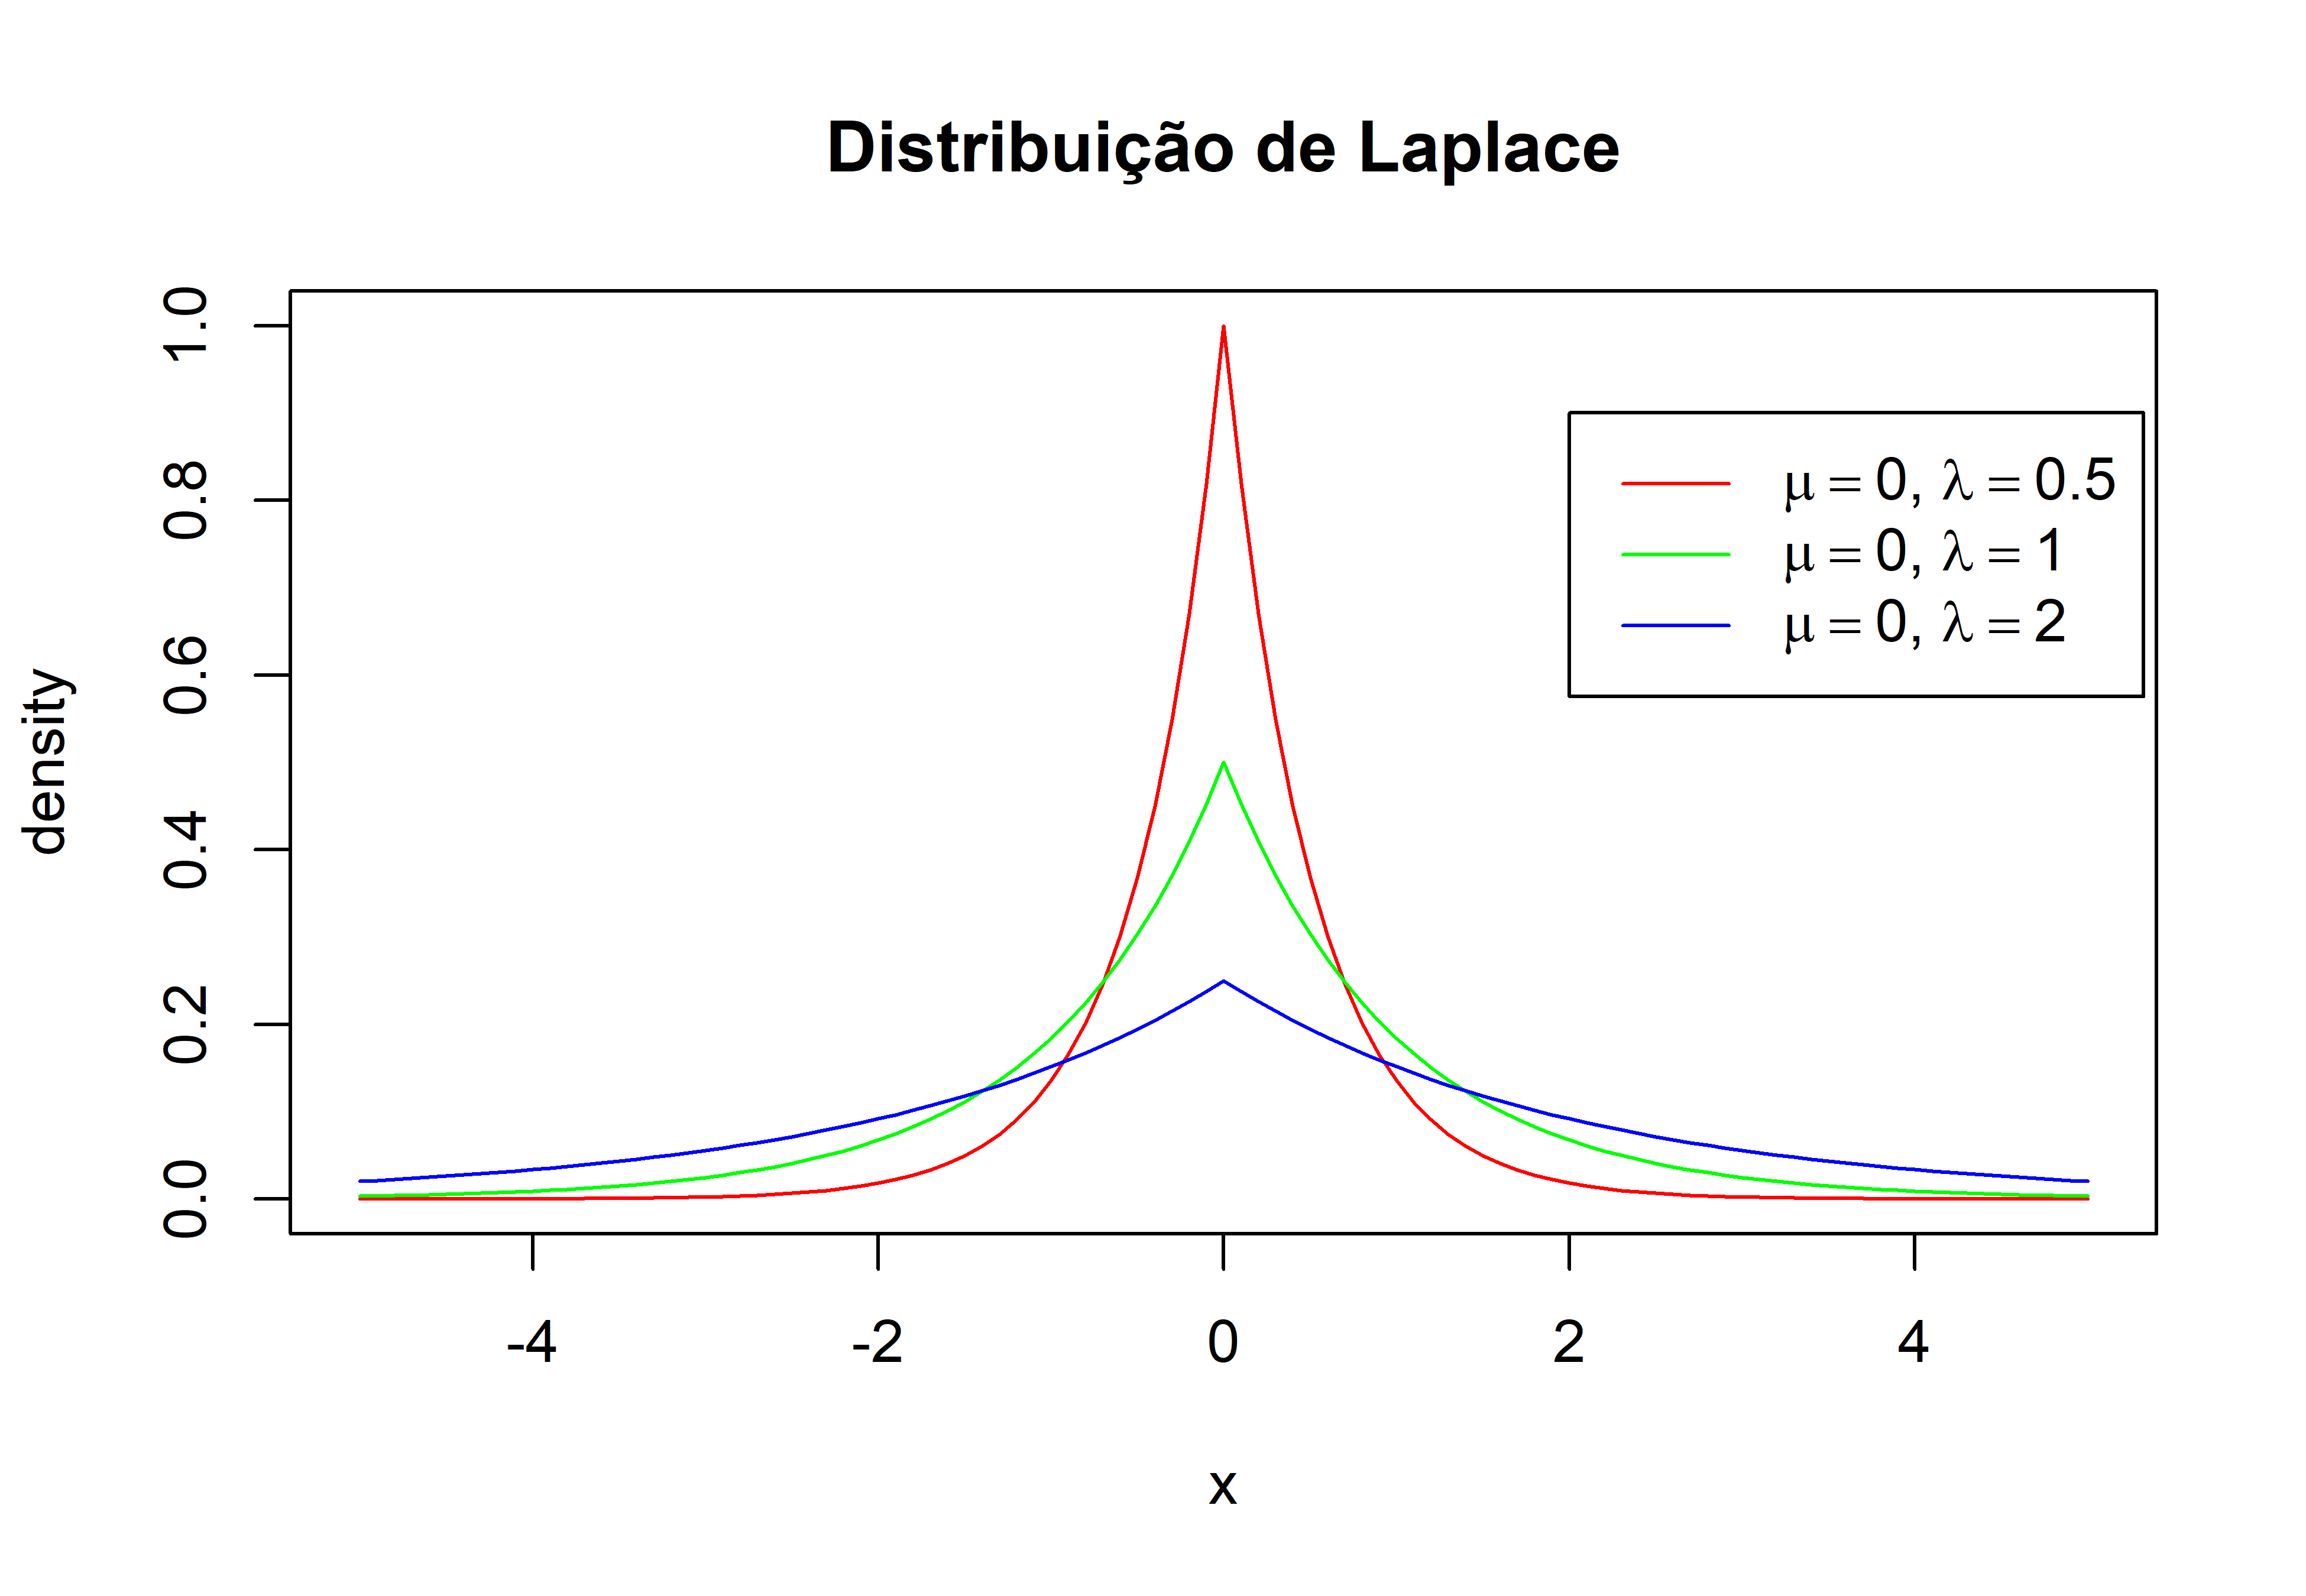
\includegraphics[width=0.7\linewidth]{images/dist_Laplace-1} 

}

\caption{Distribuição de Laplace.}\label{fig:dist_Laplace}
\end{figure}

\[\hat \mu = \arg\min_c \sum |x_i - c|\]
\[\hat \lambda = \frac{1}{n} \sum_{i=1}^n |x_i - \hat \mu|\]

\[f(x|\mu, \lambda) = \frac{1}{2 \lambda} \exp \left ( -\frac{|x - \mu|}{\lambda}\right )\]

\hypertarget{inferencia}{%
\subsection{Inferência}\label{inferencia}}

\hypertarget{aplicacoes-da-regressao-quantilica}{%
\subsection{Aplicações da regressão
quantílica}\label{aplicacoes-da-regressao-quantilica}}

\hypertarget{estudos-de-caso}{%
\section{Estudos de Caso}\label{estudos-de-caso}}

Para os estudos de caso foram utilizados os dados disponíveis em
HOCHHEIM (\protect\hyperlink{ref-hochheim}{2015}).

\hypertarget{duas-dimensoes}{%
\subsection{Duas dimensões}\label{duas-dimensoes}}

Assim como na regressão linear, é mais fácil aa compreensão da regressão
quantílica através de exemplos em duas dimensões, e depois generalizar
para \(n\) dimensões.

Seja primeiramente o caso de dados heteroscedásticos. A figura
\ref{fig:qr1} ilustra a aplicação da regressão quantílica e da regressão
linear para este caso. Na figura \ref{fig:qr1}, a reta vermelha é a reta
de regressão linear entre as variáveis. A área sombreada em cinza é o
intervalo de confiança para a regressão linear @80\%. As retas azuis são
as retas de regressão quantílica para os quantis 0,1; 0,2; 0,3; 0,4;
0,5; 0,6; 0,7; 0,8 e 0,9.

A regressão quantílica neste caso pode ser usada para demonstrar a não
validade dos intervalos de confiança (IC) e predição (IP) para a
regressão linear para este tipo de dados: como a variância da população
não é constante, mas aumenta com o aumento da área, as retas da
regressão quantílica se abrem. Como os intervalos de confiança e
predição na inferência clássica são calculados considerando-se que a
variância da população é constante, este efeito não se observa no
formato do IC.

\begin{figure}[H]

{\centering 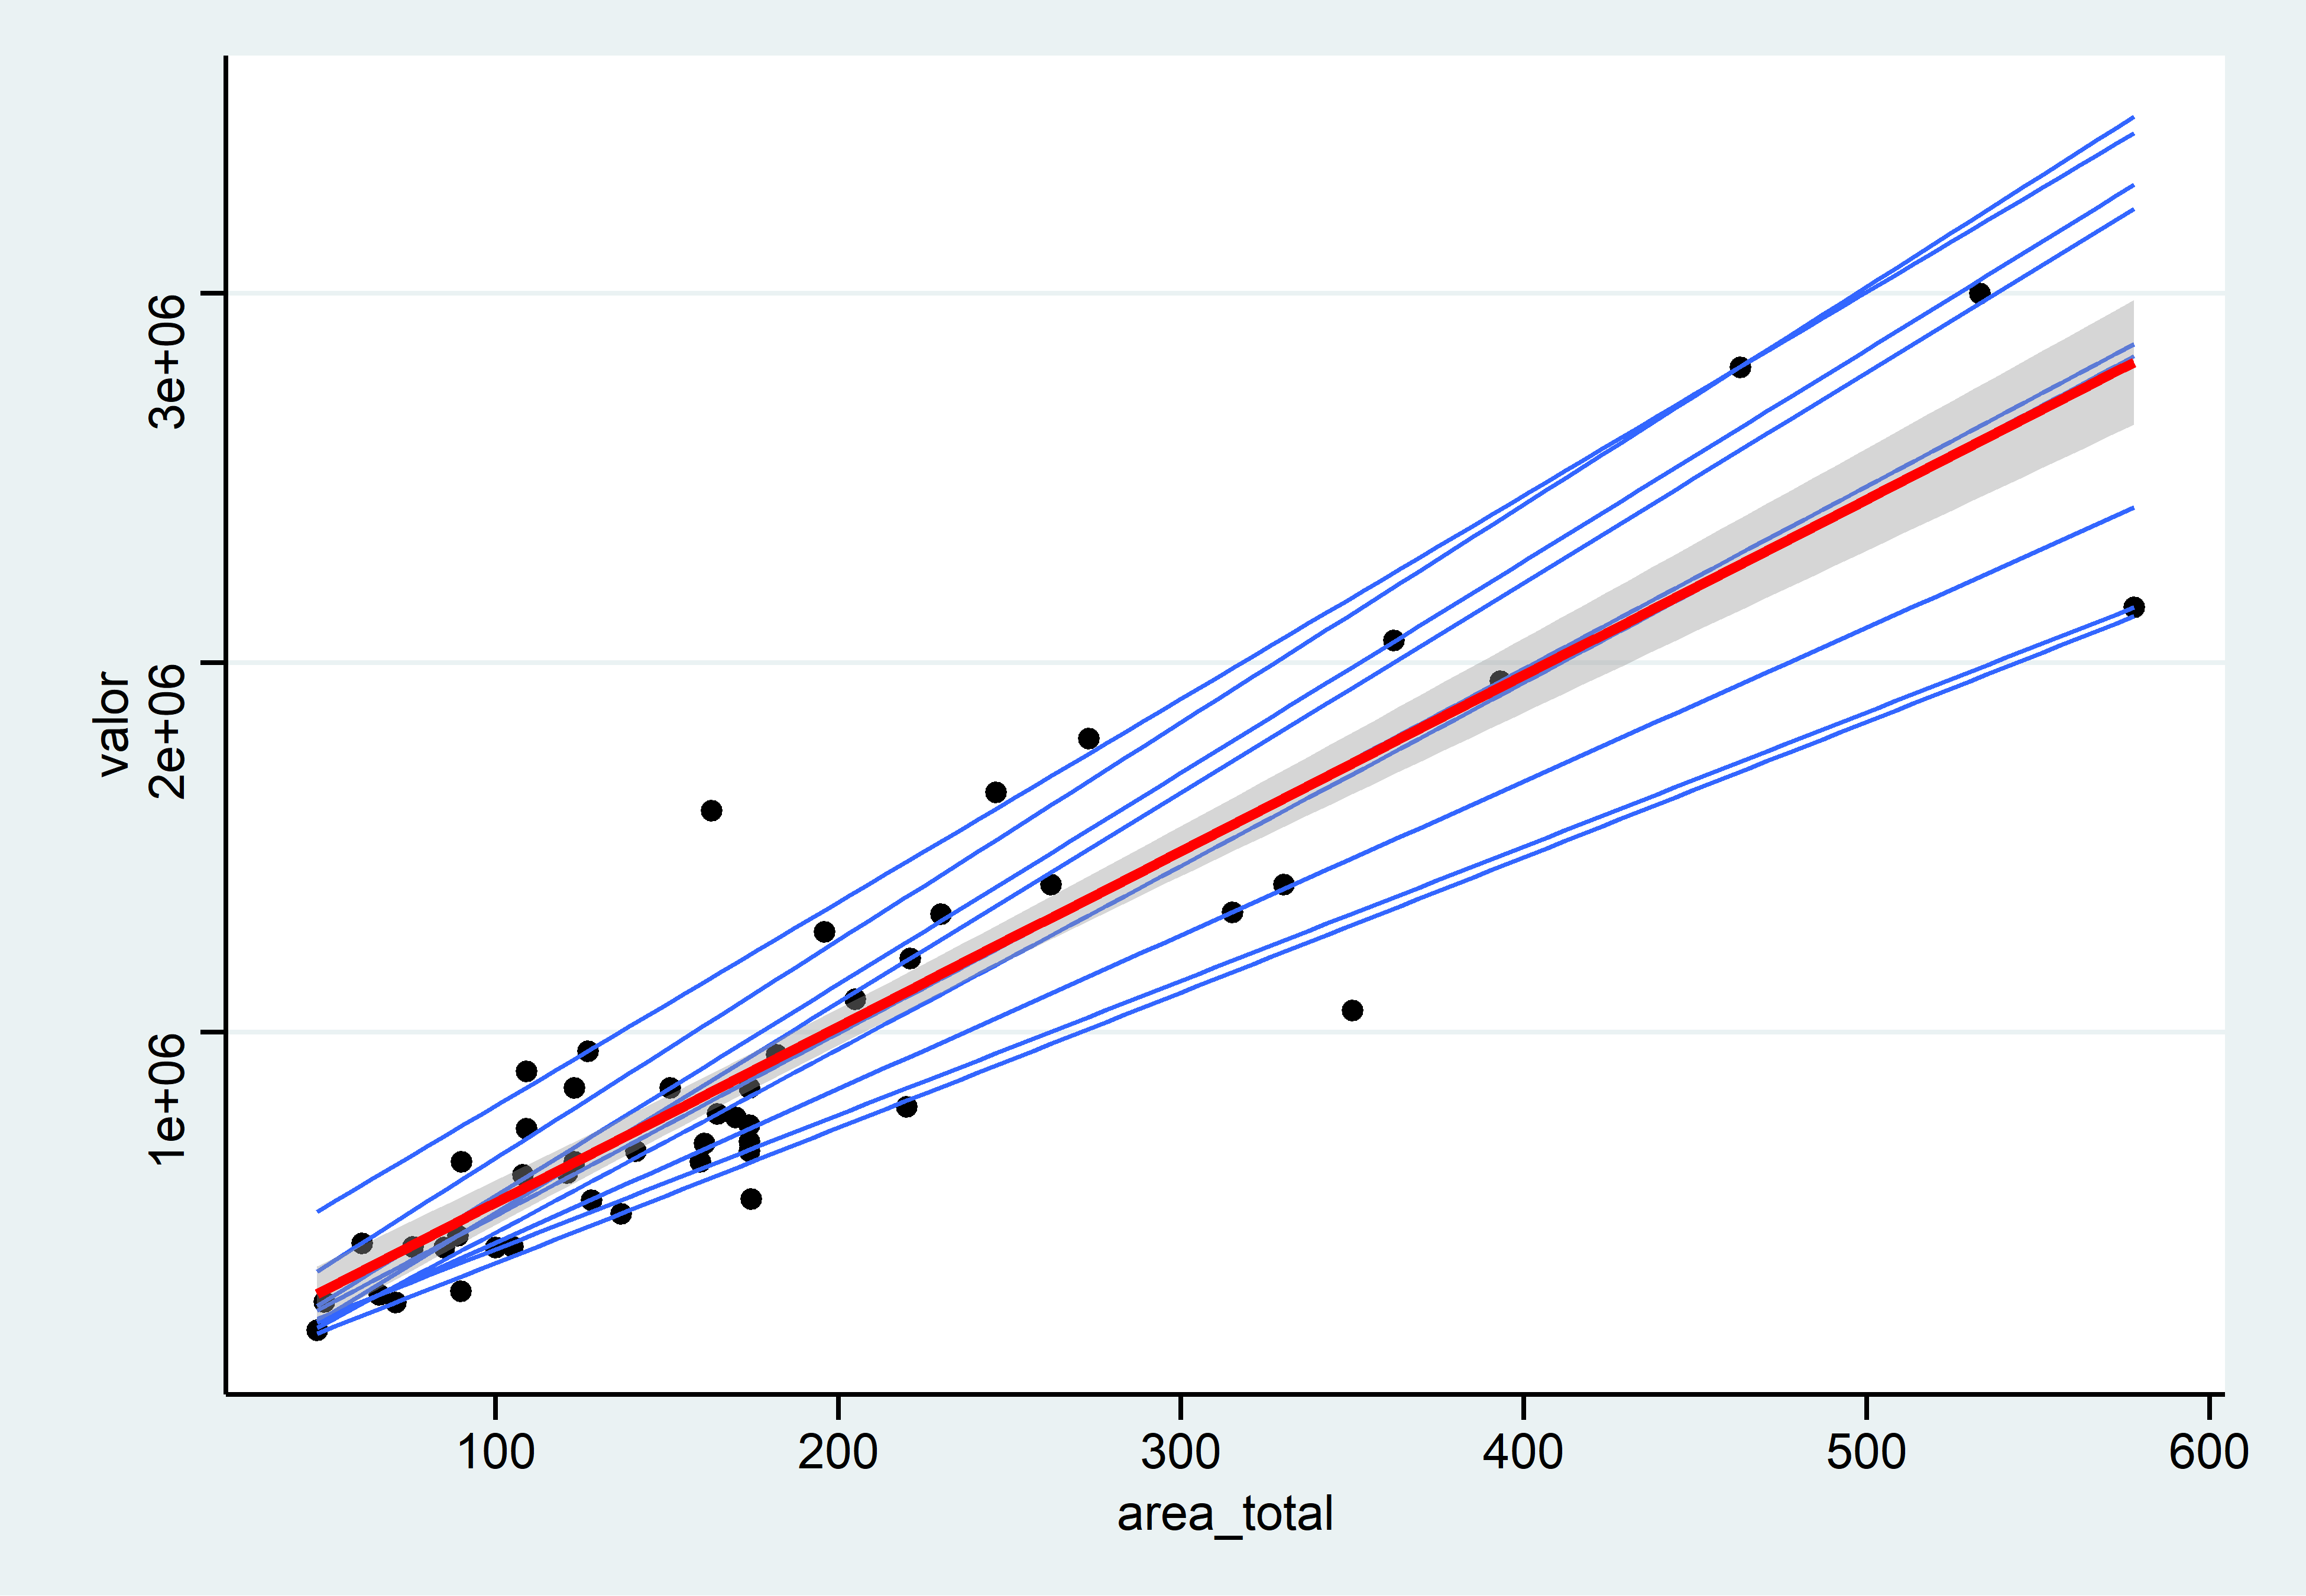
\includegraphics[width=0.7\linewidth]{images/qr1-1} 

}

\caption{Regressão Linear e Quantílica para dados heteroscedásticos.}\label{fig:qr1}
\end{figure}

Assim como na regressão linear, uma conveniente transformação das
variáveis pode ser aplicada para a obtenção da homoscedasticidade. Isto
pode ser visto na figura \ref{fig:qr2}, onde as retas para os diferentes
quantis obtidas pela regressão quantílica agora são praticamente
paralelas entre si, indicando que a heteroscedasticidade foi removida.

\begin{figure}[H]

{\centering 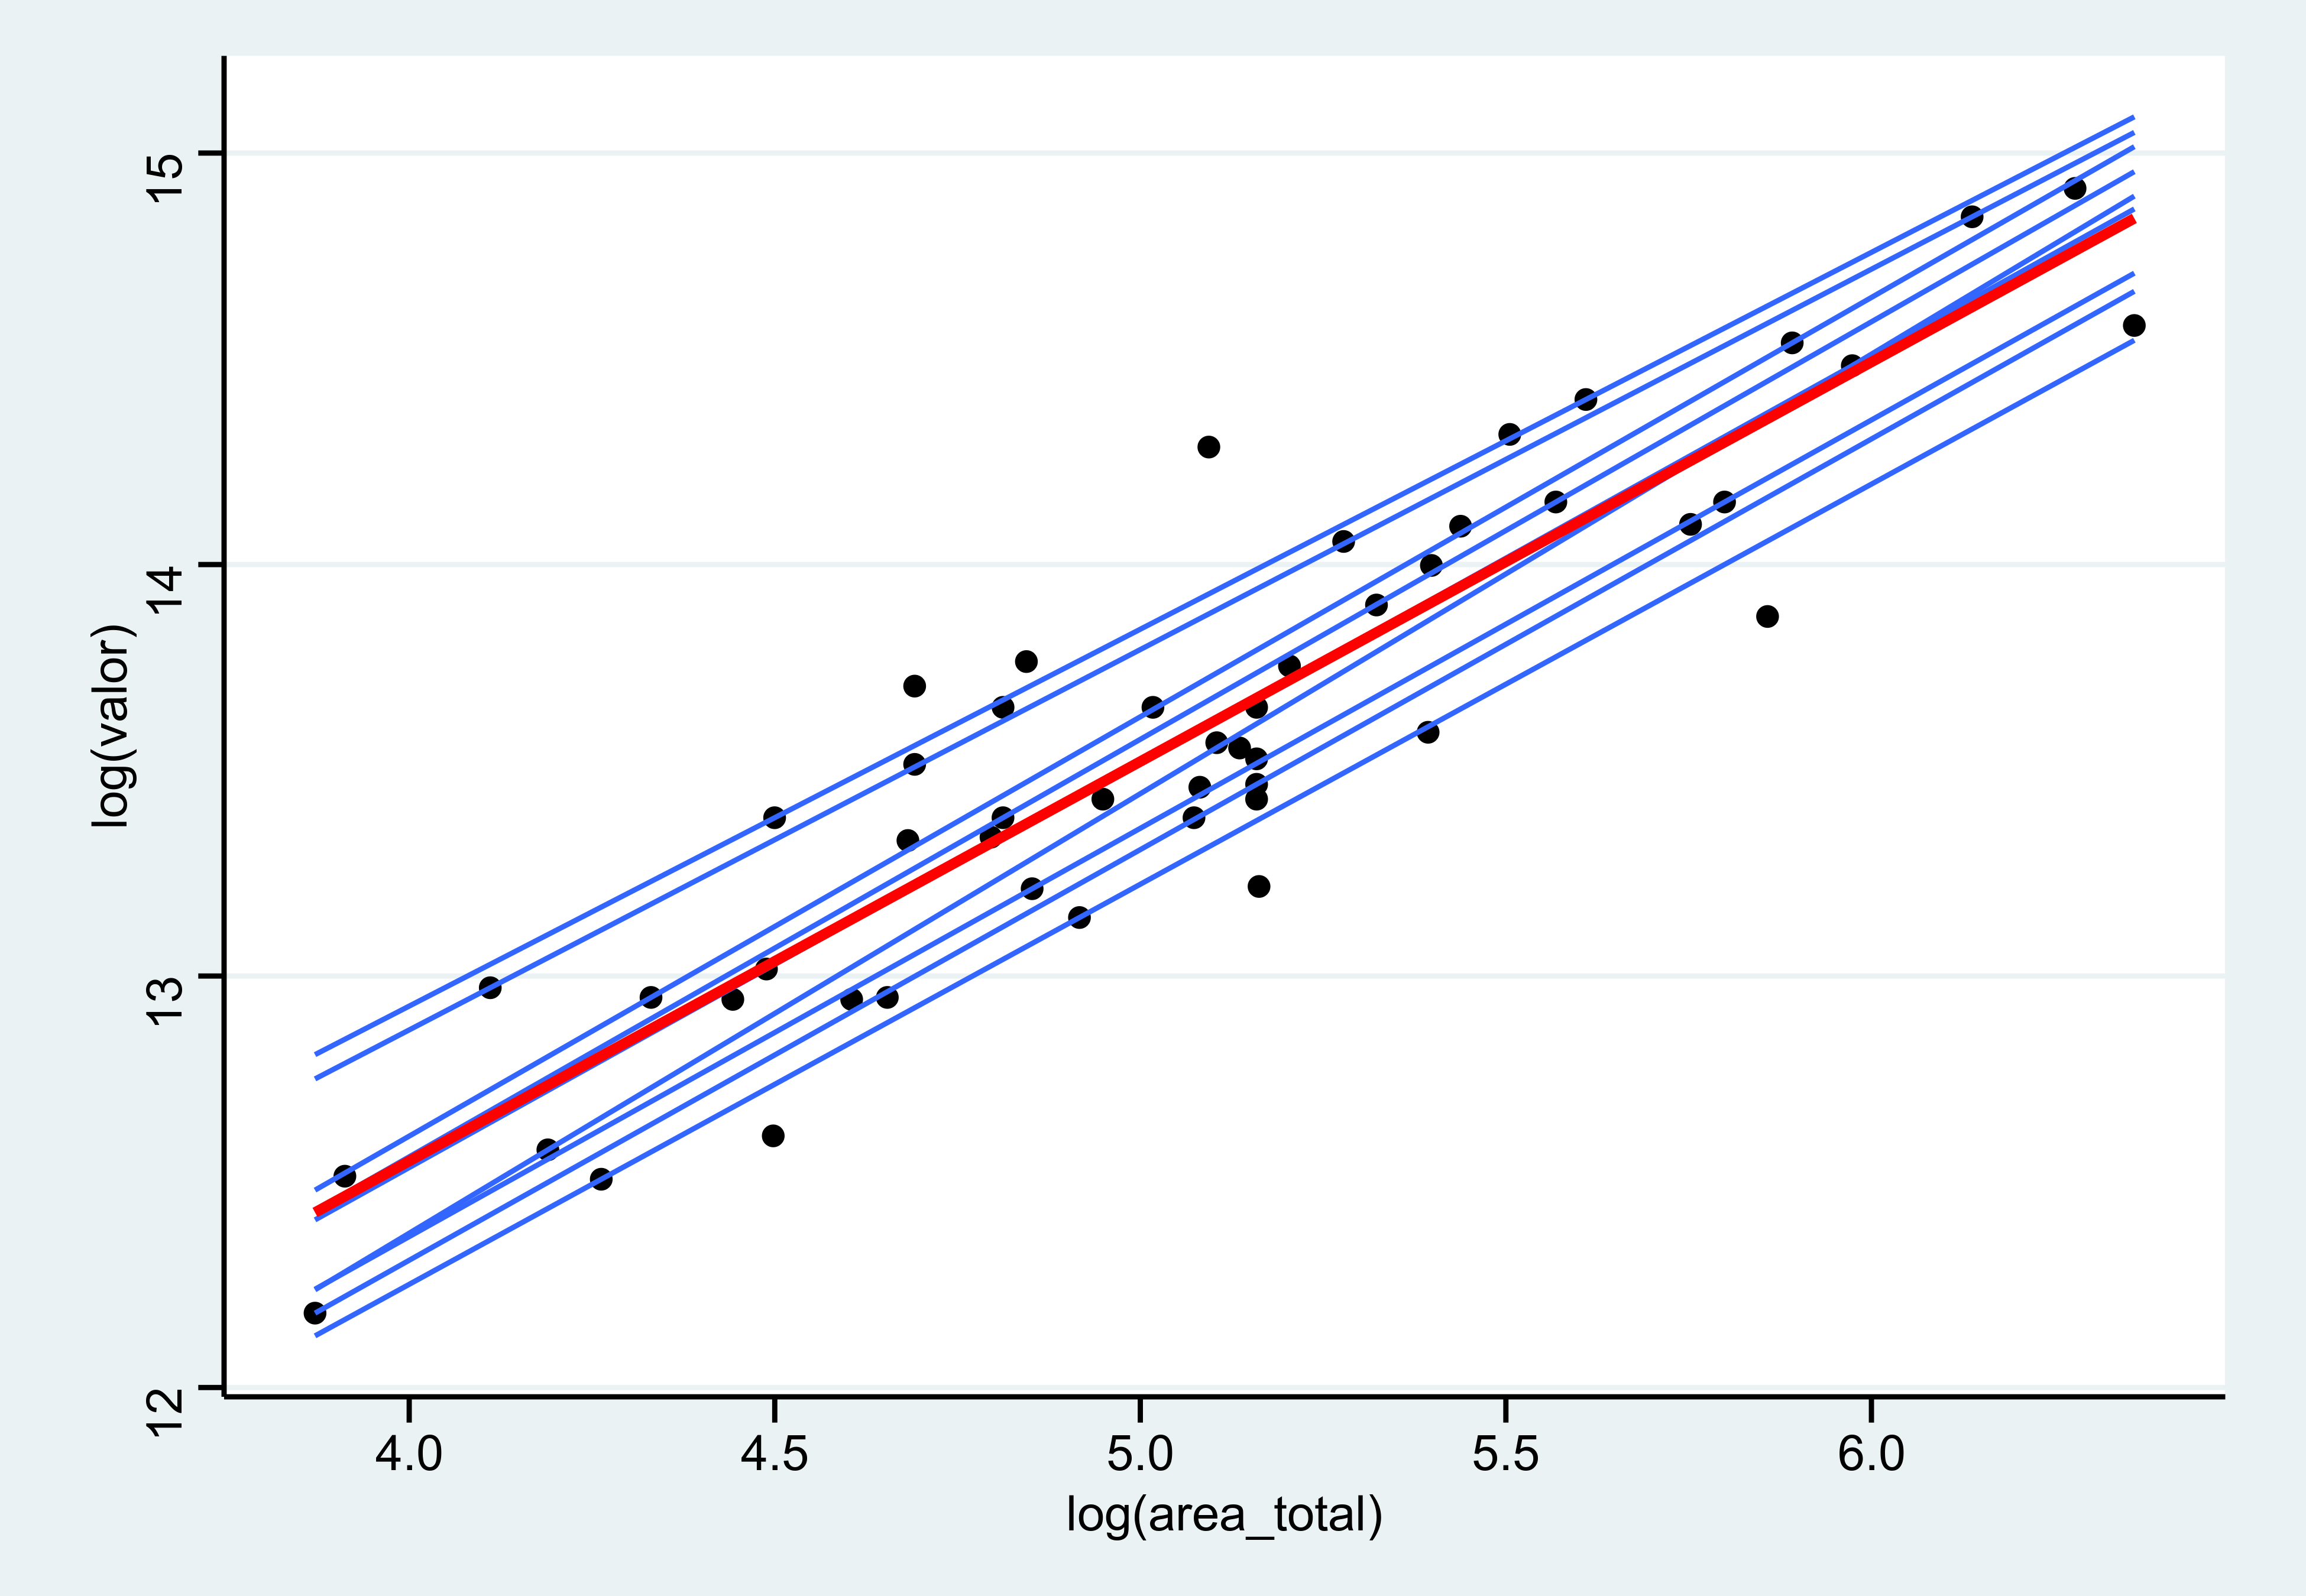
\includegraphics[width=0.7\linewidth]{images/qr2-1} 

}

\caption{Regressão Linear e Quantílica com dados transformados.}\label{fig:qr2}
\end{figure}

Os coeficientes das retas de regressão quantílica podem ser plotados
como na figura \ref{fig:coef1}. Nesta figura, a reta cheia vermelha
representa o coeficiente do modelo de regressão linear, enquanto a reta
preta pontilhada representa os vários coeficientes da regressão
quantílica. As retas vermelhas tracejadas representam o intervalo de
confiança de estimação do coeficiente de regressão linear. A área
sombreada em cinza representa os intervalos de confiança para os
coeficientes da regressão quantílica. Deve-se notar que, entre os
quantis aproximados de 0,3 e 0,55, os coeficientes da regressão
quantílica não são significamente diferentes, estatísticamente, do
coeficiente da regreessão linear.

\begin{figure}[H]

{\centering 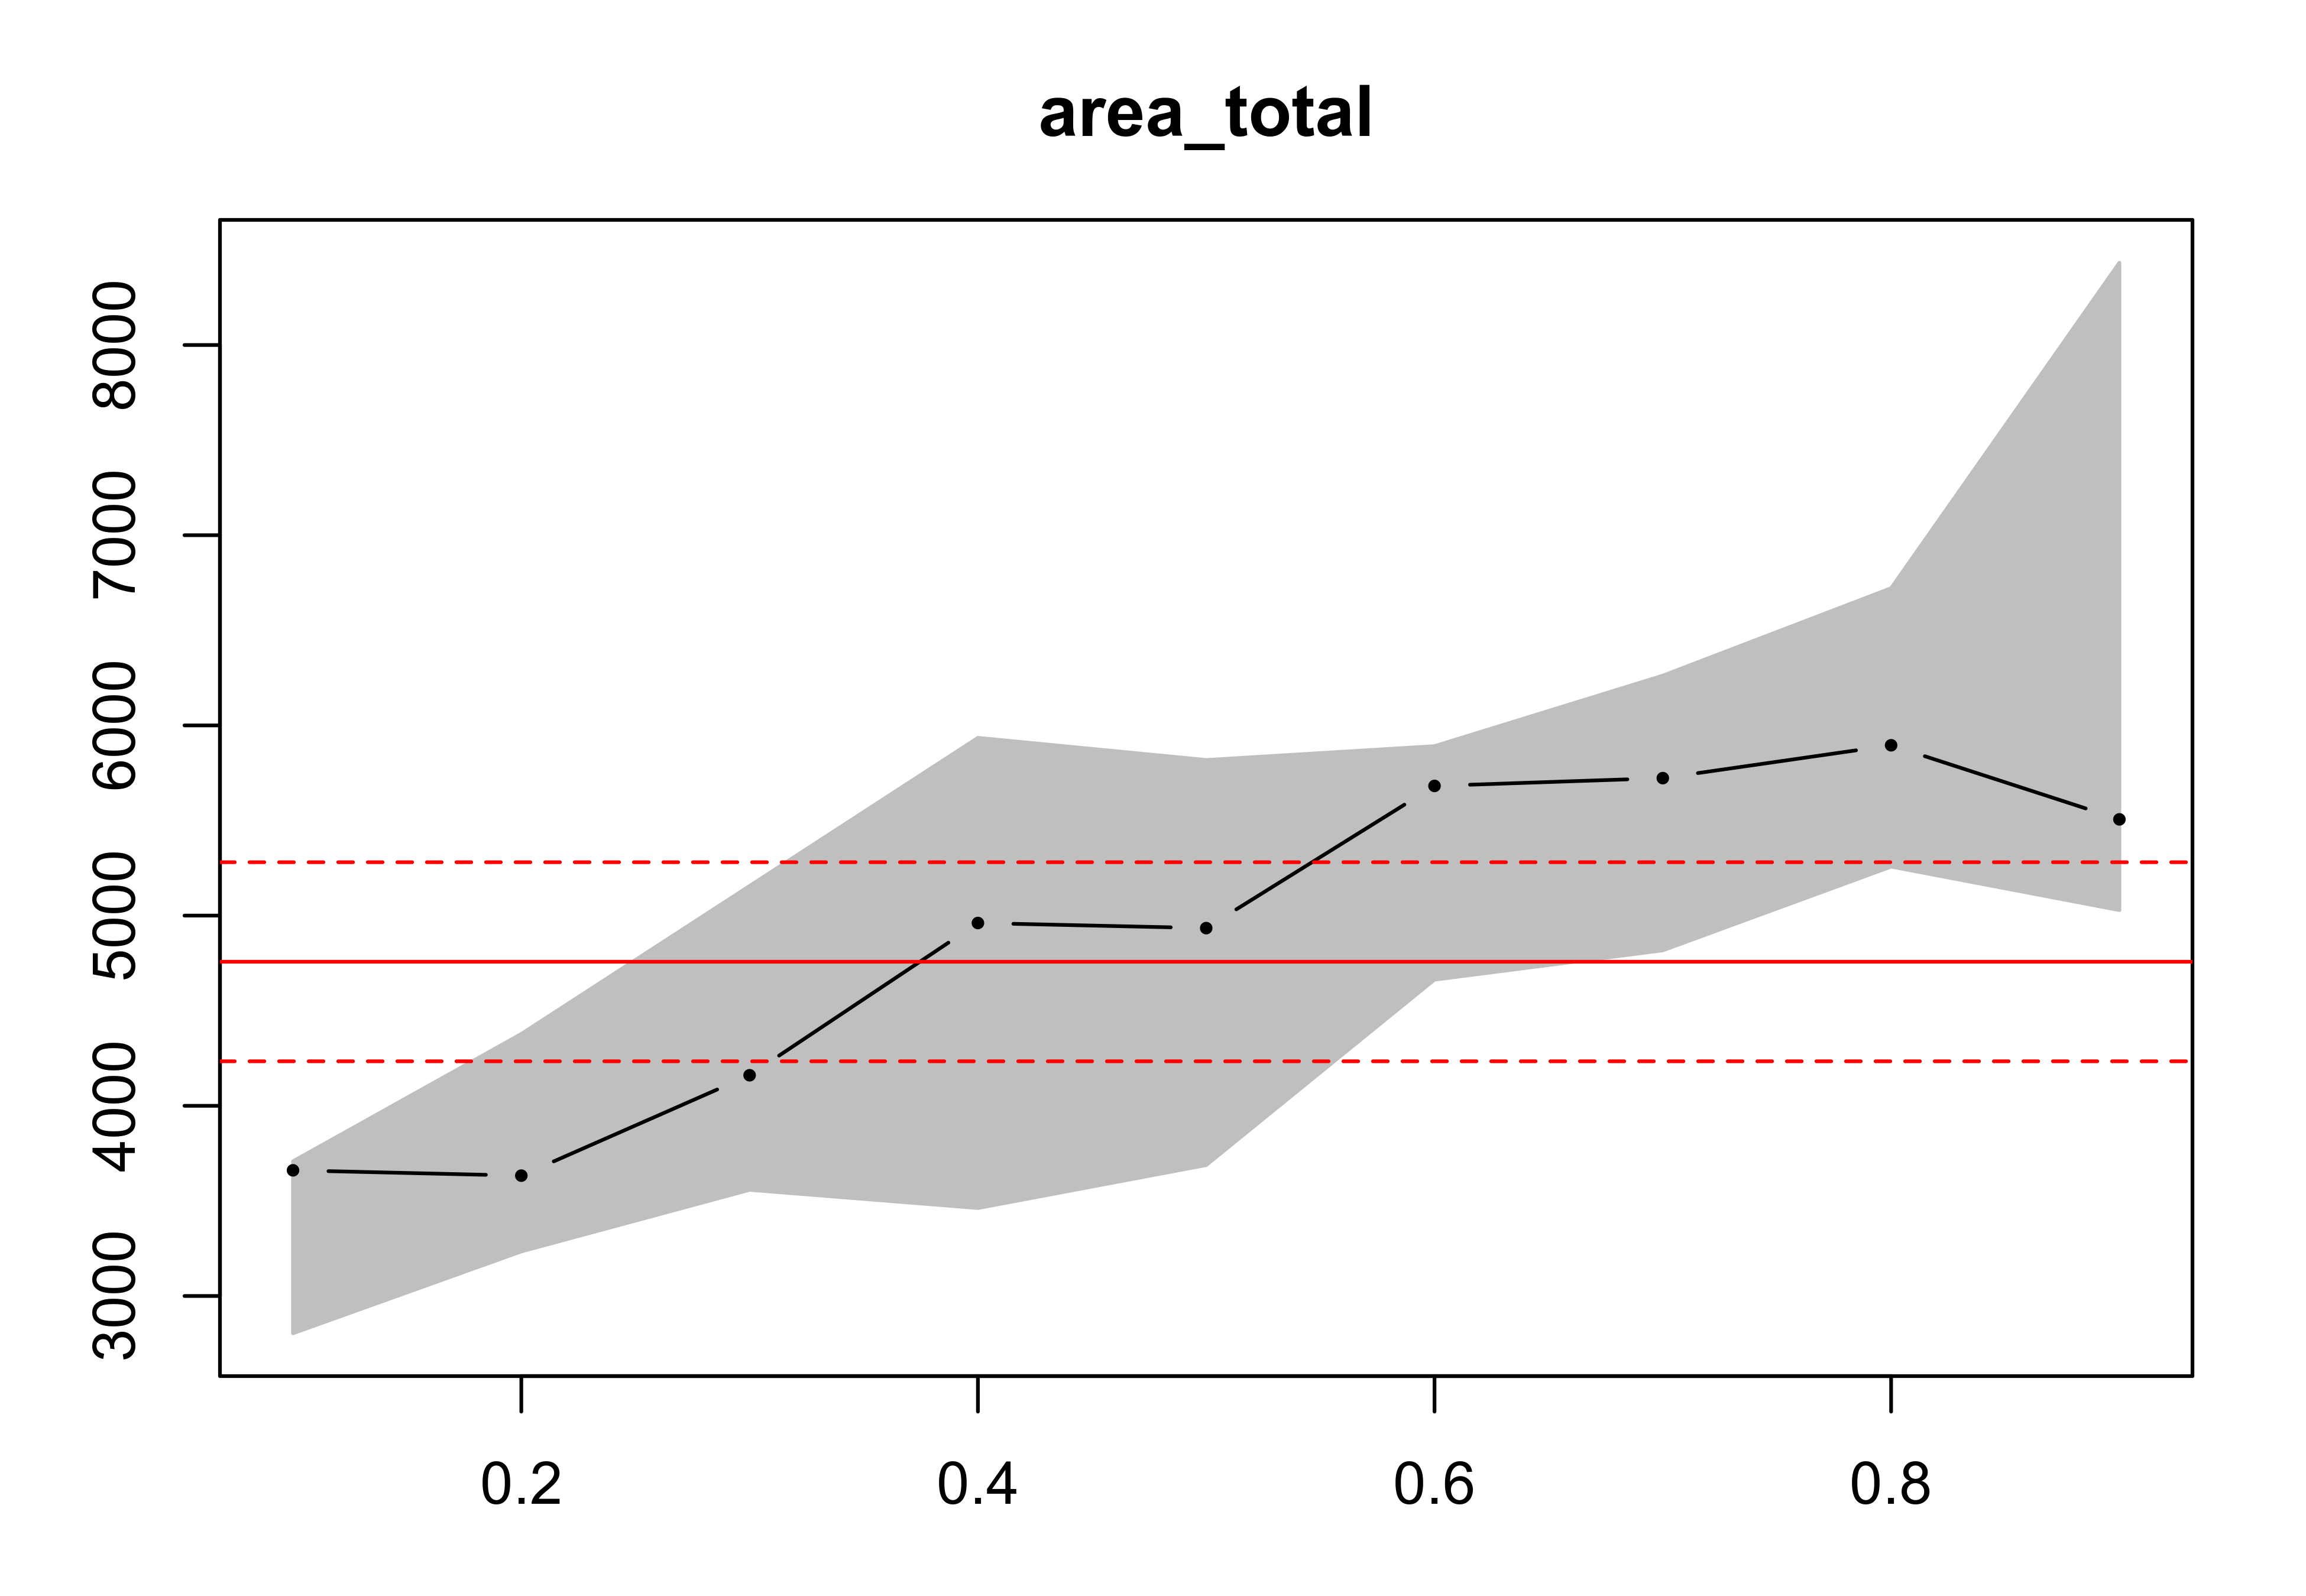
\includegraphics[width=0.7\linewidth]{images/coef1-1} 

}

\caption{Variação dos coeficientes de regressão quantílica (variáveis originais).}\label{fig:coef1}
\end{figure}

Já para os dados transformados, pode-se notar na figura \ref{fig:coef2}
que para todos os quantis, os coeficientes da regressão quantílica não
podem ser considerados estatisticamente diferentes do coeficiente da
regressão linear. Também se pode notar nesta figura como o estimador de
regressão linear, para uma variável normalmente distribuída e na
ausência de heteroscedasticidade, é mais eficiente do que o estimador da
regressão quantílica, como a teoria já prevê (ver MATLOFF
(\protect\hyperlink{ref-matloff2017}{2017}), 238).

(Zilli, não sei se tu pesquisou isso na revisão bibliográfica, mas acho
que se não, era bom colocar! Colocar algo do tipo: as vantagens e
desvantagens da regressão quantílica. Apesar da regressão quantílica ser
robusta à presença de \emph{outliers}, ela é menos eficiente do que a
regressao linear, caso a distribuição da variável estudada seja normal,
claro.)

\begin{figure}[H]

{\centering 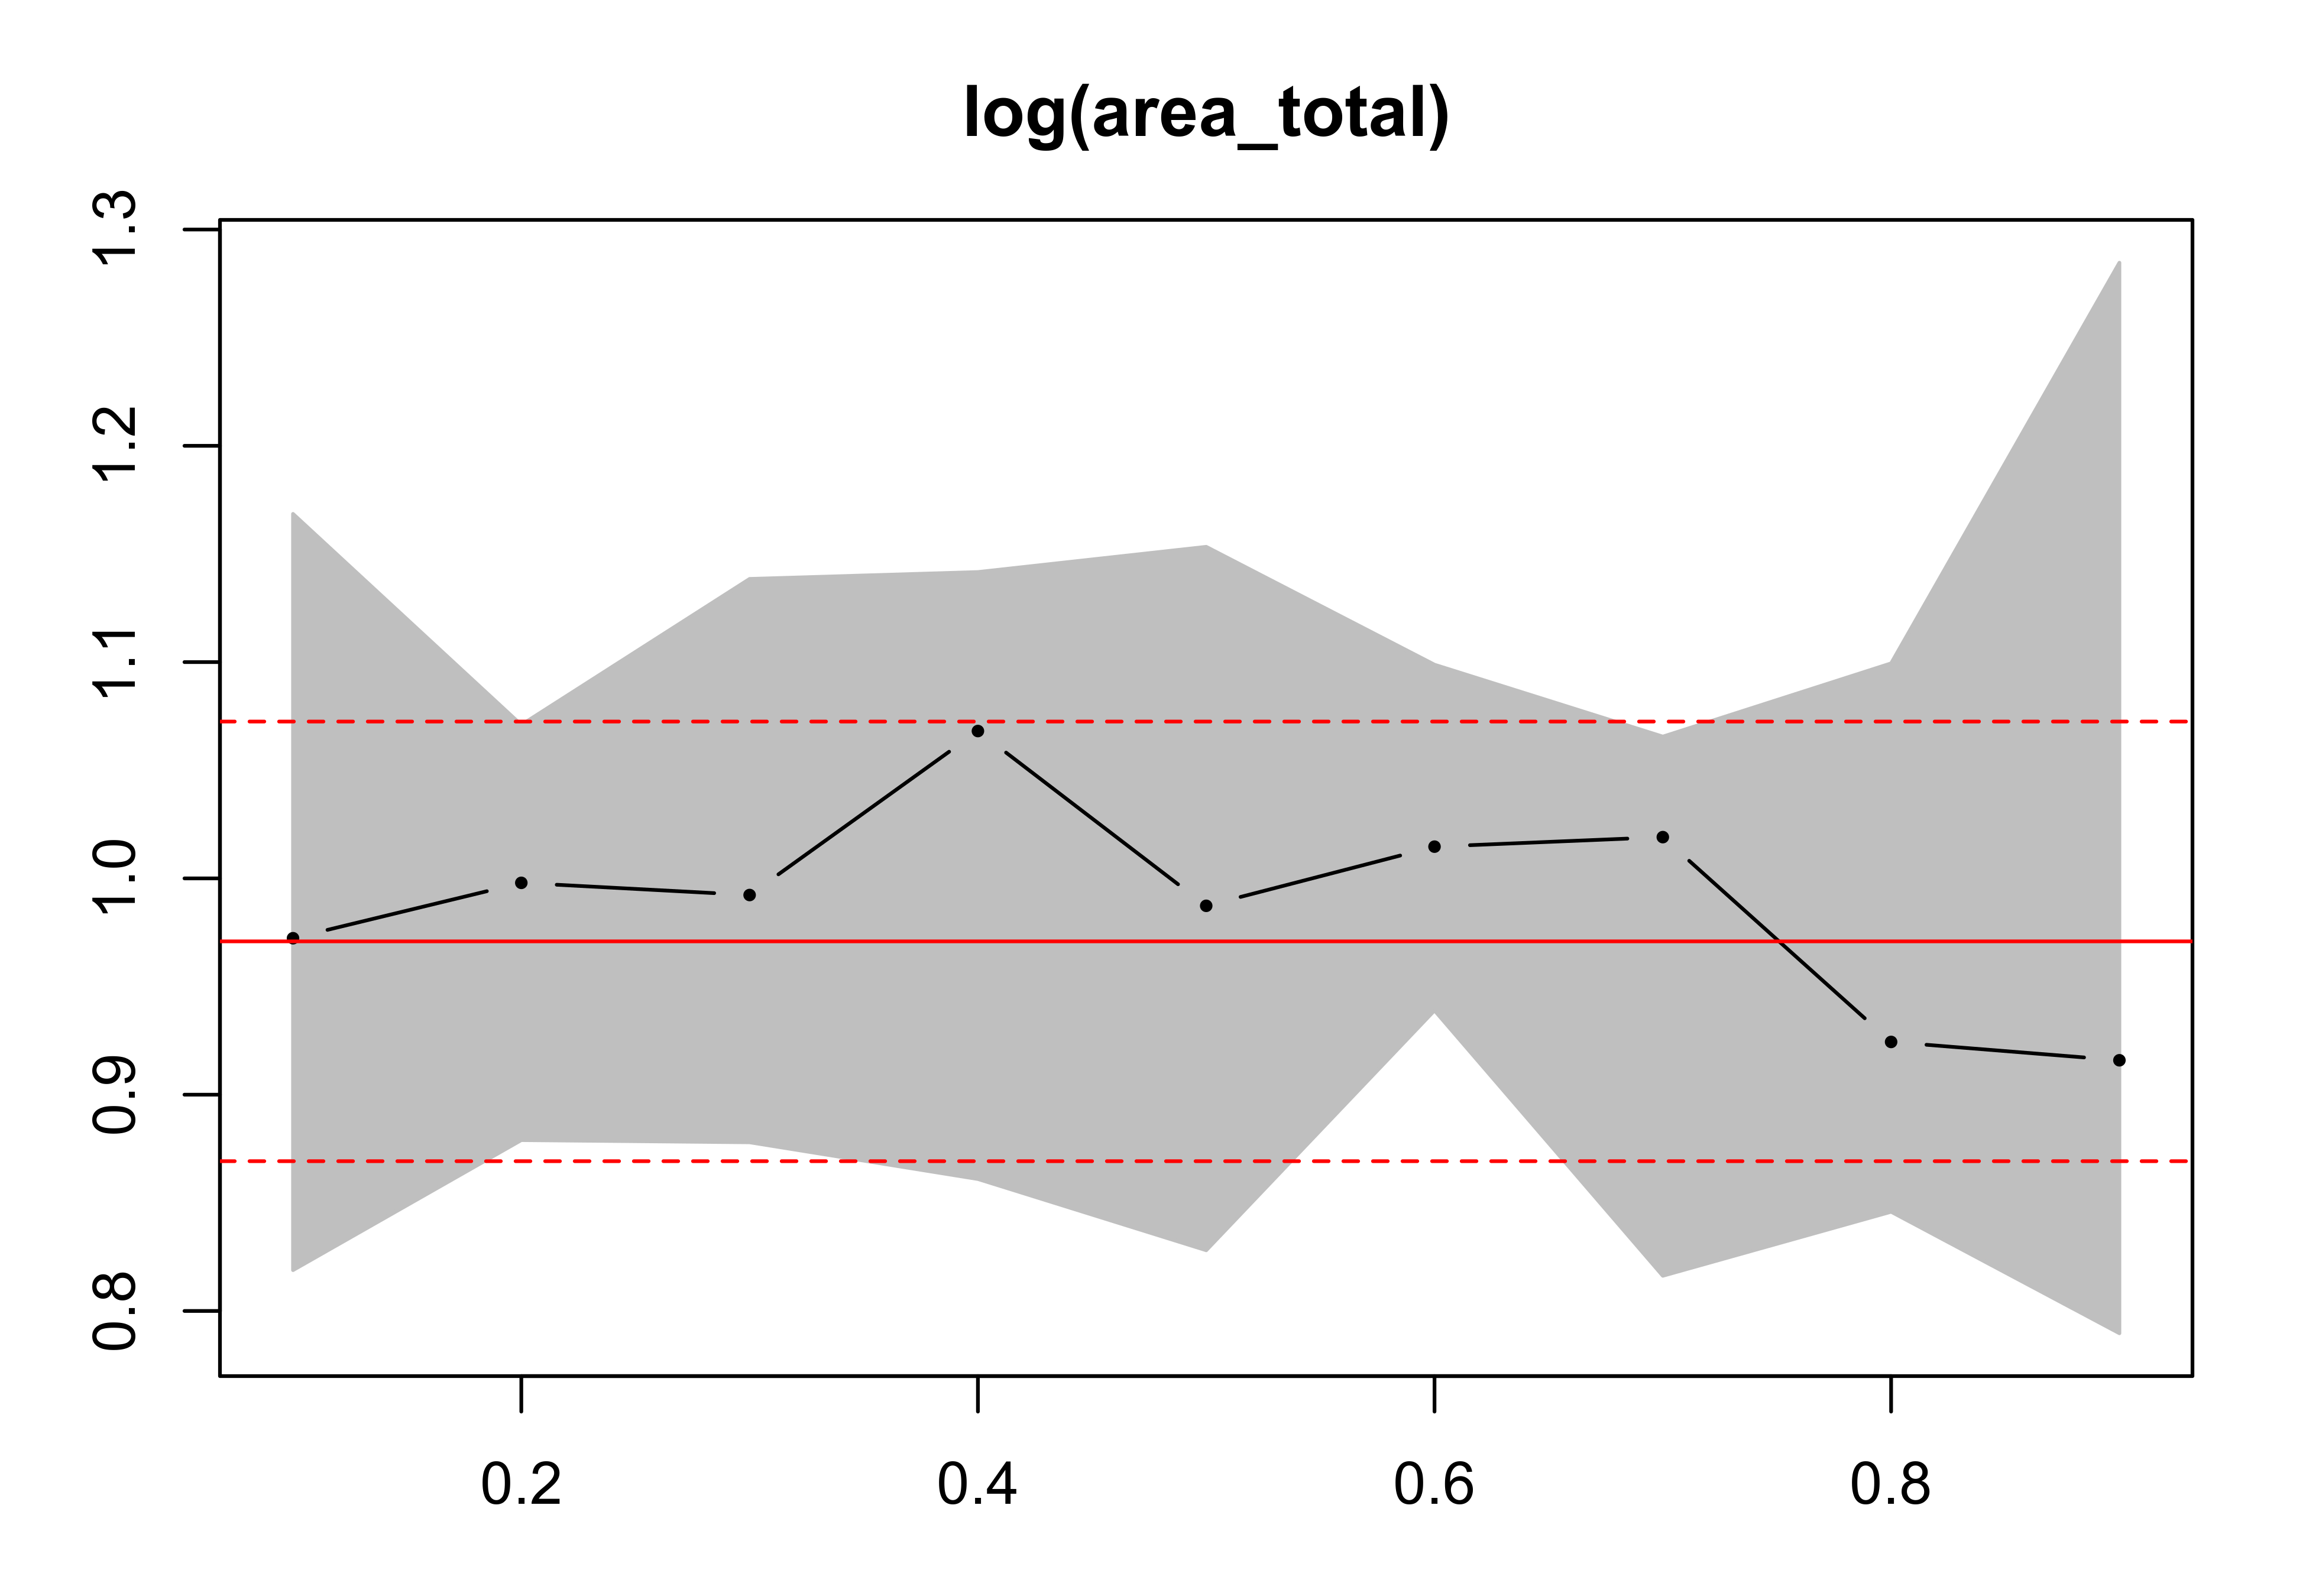
\includegraphics[width=0.7\linewidth]{images/coef2-1} 

}

\caption{Variação dos coeficientes de regressão quantílica (variáveis transformadas).}\label{fig:coef2}
\end{figure}

\hypertarget{analise-multivariada}{%
\subsection{Análise Multivariada}\label{analise-multivariada}}

Para os dados obtidos de Hochheim
(\protect\hyperlink{ref-hochheim}{2015}, pp. 22--23) foram ajustados
dois modelos, um de regressão linear, com os dados saneados, e outro de
regressão quantílica, utilizando-se a totalidade dos dados, para os
quantis 0,1; 0,2; 0,3; 0,4; 0,5; 0,6; 0,7; 0,8 e 0,9.

Na figura \ref{fig:coefs} podem ser vistos os valores dos coeficientes
de cada variável para os diferentes quantis. Pode-se perceber, mais uma
vez, que o valor dos coeficientes da regressão quantílica não diferem
significantemente dos coeficientes da regressão linear (exceção para
alguns quantis superiores nas variáveis \texttt{area\_total} e
\texttt{padrao}).

\begin{figure}[H]

{\centering 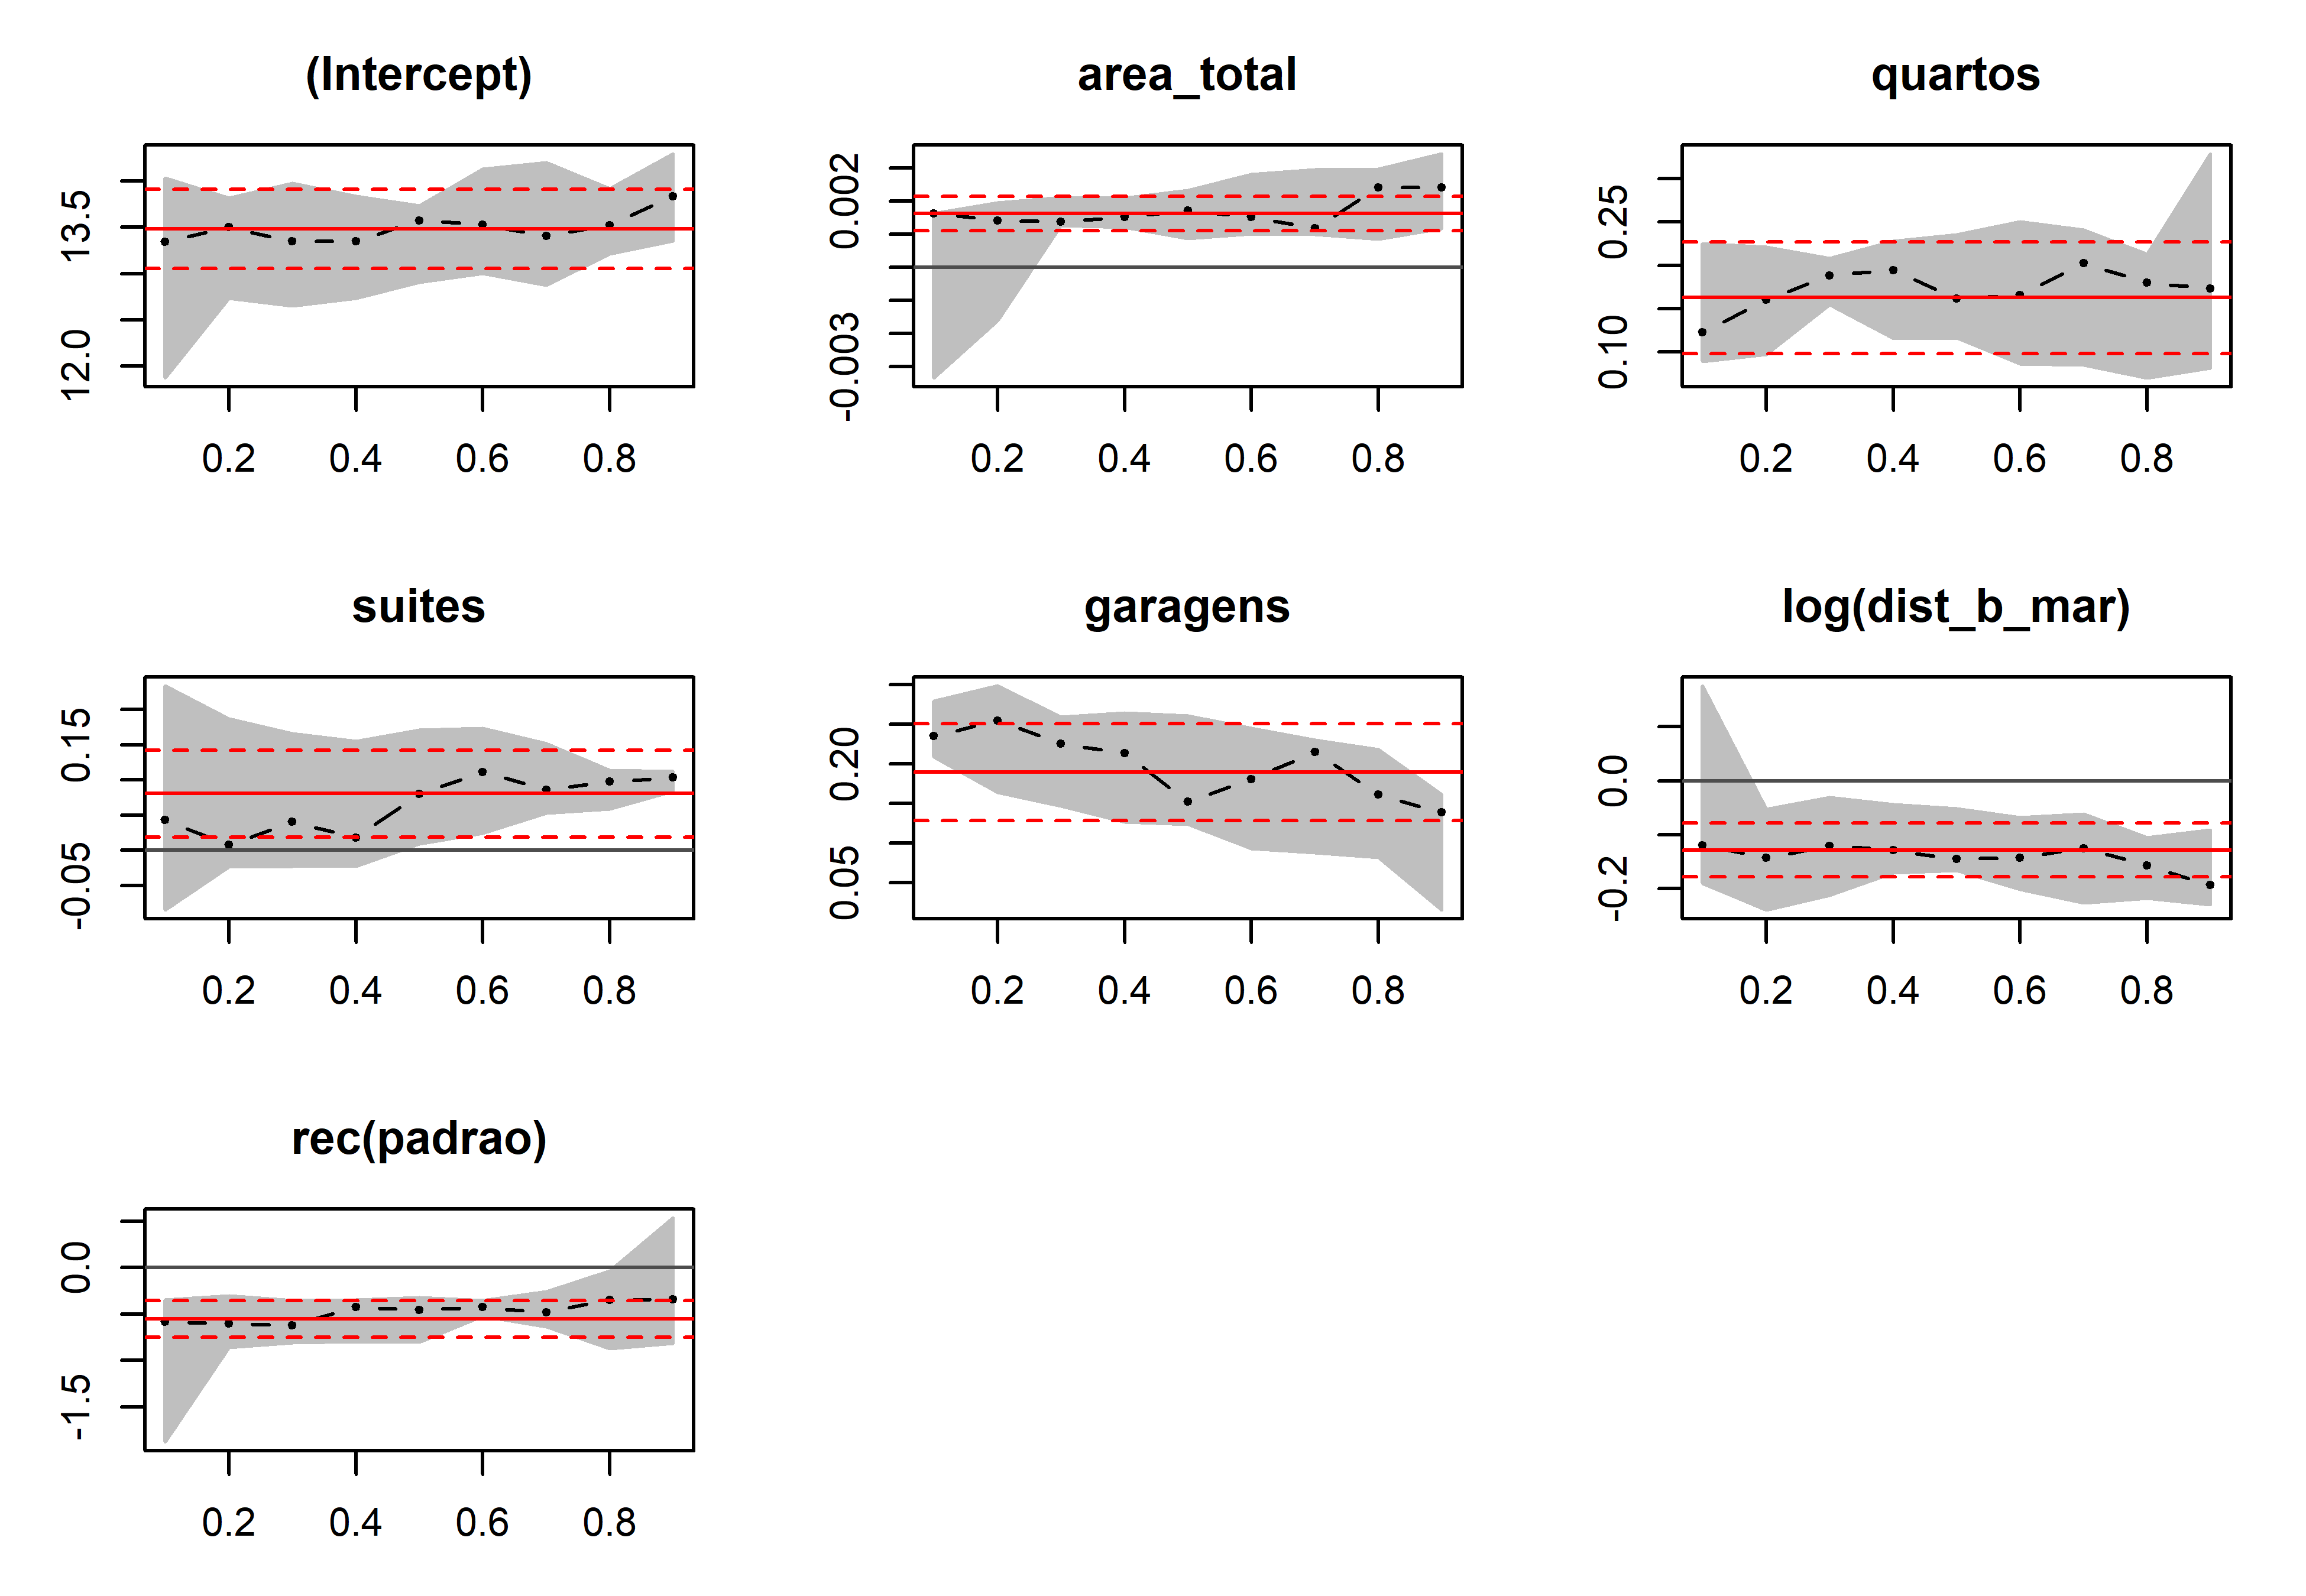
\includegraphics[width=1\linewidth]{images/coefs-1} 

}

\caption{Coeficientes de regressão linear e quantílica. Análise multivariada.}\label{fig:coefs}
\end{figure}

Na tabela \ref{tab:fits} podem ser vistos os coeficientes e estatísticas
básicas dos modelos de regressão linear e de regressão à mediana
(quantil 0,5).

\begin{table}[!htbp] \centering 
  \caption{Comparação entre os modelos de regressão linear e regressão à mediana.} 
  \label{tab:fits} 
\begin{tabular}{@{\extracolsep{5pt}}lcc} 
\\[-1.8ex]\hline 
\hline \\[-1.8ex] 
 & \multicolumn{2}{c}{\textit{Dependent variable:}} \\ 
\cline{2-3} 
\\[-1.8ex] & \multicolumn{2}{c}{log(valor)} \\ 
\\[-1.8ex] & \textit{OLS} & \textit{quantile} \\ 
 & \textit{} & \textit{regression} \\ 
\\[-1.8ex] & (1) & (2)\\ 
\hline \\[-1.8ex] 
 area\_total & 0.001 & 0.002 \\ 
  & (0.001, 0.002) & (0.001, 0.003) \\ 
  & t = 5.113 & t = 2.300 \\ 
  & p = 0.00001$^{***}$ & p = 0.027$^{**}$ \\ 
  & & \\ 
 quartos & 0.164 & 0.162 \\ 
  & (0.118, 0.209) & (0.107, 0.217) \\ 
  & t = 4.626 & t = 3.788 \\ 
  & p = 0.00004$^{***}$ & p = 0.0005$^{***}$ \\ 
  & & \\ 
 suites & 0.061 & 0.080 \\ 
  & (0.018, 0.104) & (0.020, 0.139) \\ 
  & t = 1.810 & t = 1.712 \\ 
  & p = 0.078$^{*}$ & p = 0.095$^{*}$ \\ 
  & & \\ 
 garagens & 0.209 & 0.152 \\ 
  & (0.166, 0.252) & (0.075, 0.230) \\ 
  & t = 6.247 & t = 2.520 \\ 
  & p = 0.00000$^{***}$ & p = 0.016$^{**}$ \\ 
  & & \\ 
 log(dist\_b\_mar) & $-$0.141 & $-$0.146 \\ 
  & ($-$0.176, $-$0.106) & ($-$0.210, $-$0.081) \\ 
  & t = $-$5.174 & t = $-$2.904 \\ 
  & p = 0.00001$^{***}$ & p = 0.006$^{***}$ \\ 
  & & \\ 
 rec(padrao) & $-$0.563 & $-$0.459 \\ 
  & ($-$0.697, $-$0.428) & ($-$0.650, $-$0.267) \\ 
  & t = $-$5.360 & t = $-$3.070 \\ 
  & p = 0.00001$^{***}$ & p = 0.004$^{***}$ \\ 
  & & \\ 
 Constant & 13.564 & 13.574 \\ 
  & (13.268, 13.859) & (13.100, 14.047) \\ 
  & t = 58.847 & t = 36.732 \\ 
  & p = 0.000$^{***}$ & p = 0.000$^{***}$ \\ 
  & & \\ 
\hline \\[-1.8ex] 
Observations & 48 & 50 \\ 
R$^{2}$ & 0.956 &  \\ 
Adjusted R$^{2}$ & 0.950 &  \\ 
Residual Std. Error & 0.136 (df = 41) &  \\ 
F Statistic & 148.921$^{***}$ (df = 6; 41) &  \\ 
\hline 
\hline \\[-1.8ex] 
\textit{Note:}  & \multicolumn{2}{r}{$^{*}$p$<$0.1; $^{**}$p$<$0.05; $^{***}$p$<$0.01} \\ 
\end{tabular} 
\end{table}

\hypertarget{estimativas}{%
\subsubsection{Estimativas}\label{estimativas}}

É interessante comparar as estimativas obtidas com os modelos de
regressão linear, com dados saneados, e o modelo de regressão à mediana,
com a totalidade dos dados. Por um lado, o modelo de regressão linear
tende a ser mais preciso para a estimação da média, como prevê a teoria.
Por outro lado, com mais dados, o modelo de regressão à mediana pode
tornar-se mais eficiente.

Deve-se levar em conta que as estimativas com o modelo de regressão
linear aqui apresentadas são para a mediana da distribuição lognormal.

Pelo modelo de regressão linear, o valor da estimativa central
encontrado foi de R\$961.660,64, com intervalo de confiança entre R\$
924.768,13 e R\$ 1.000.024,94. A amplitude do intervalo de confiança foi
de 7.83\%.

Já pelo modelo de regressão quantílica, o valor da estimativa central
encontrado foi de R\$946.467,87, com intervalo de confiança entre R\$
886.472,34 e R\$ 1.010.523,85. A amplitude do intervalo de confiança foi
de 13.1\%.

O modelo de regressão linear mostrou-se, portanto, mais eficiente do que
o modelo de regressão a mediana, apesar no menor número de dados.

Os limites inferior e superior do intervalo de predição @80\% para o
modelo de regressão linear são, respectivamente: R\$ 802.017,63 e R\$
1.153.080,88.

Para o modelo de regressão quantílica, o intervalo de predição não faz
qualquer sentido. No entanto, é possível estimar os valores diretamente
para os quantis 0,1 e 0,9 da população. Nesta caso, os valores
encontrados foram, respectivamente: R\$ 810.629,32 e R\$ 1.186.954,14.

Podem ainda ser calculados os intervalos de confiança @80\% para as
estimativas dos quantis 0,1 e 0,9.

Os limites inferior e superior do IC para o quantil 0,1 são,
respectivamente: R\$ 781.253,06 e R\$ 841.110,17.

Os limites inferior e superior do IC para o quantil 0,9 são,
respectivamente: R\$ 1.116.547,53 e R\$ 1.261.800,41.

\hypertarget{referencias}{%
\section*{Referências}\label{referencias}}
\addcontentsline{toc}{section}{Referências}

\hypertarget{refs}{}
\leavevmode\hypertarget{ref-hochheim}{}%
HOCHHEIM, N. \textbf{Engenharia de avaliações - módulo básico}.
Florianópolis: IBAPE - SC, 2015.

\leavevmode\hypertarget{ref-koenker2000}{}%
KOENKER, R. Galton, edgeworth, frisch, and prospects for quantile
regression in econometrics. \textbf{Journal of Econometrics}, v. 95, n.
2, p. 347--374, 2000. Disponível em:
\textless{}\url{http://www.sciencedirect.com/science/article/pii/S0304407699000433}\textgreater{}..

\leavevmode\hypertarget{ref-mim}{}%
KOENKER, R. The median is the message: Wilson and hilfertys experiments
on the law of errors. \textbf{The American Statistician}, v. 63, n. 1,
p. 20--25, 2009. Taylor \& Francis. Disponível em:
\textless{}\url{https://doi.org/10.1198/tast.2009.0004}\textgreater{}..

\leavevmode\hypertarget{ref-qr}{}%
KOENKER, R.; HALLOCK, K. F. Quantile regression. \textbf{Journal of
Economic Perspectives}, v. 15, n. 4, p. 143--156, 2001. Disponível em:
\textless{}\url{http://www.aeaweb.org/articles?id=10.1257/jep.15.4.143}\textgreater{}..

\leavevmode\hypertarget{ref-koenker1978}{}%
KOENKER, R. W.; BASSETT, G. Regression quantiles. \textbf{Econometrica},
v. 46, n. 1, p. 33--50, 1978. Disponível em:
\textless{}\url{https://EconPapers.repec.org/RePEc:ecm:emetrp:v:46:y:1978:i:1:p:33-50}\textgreater{}..

\leavevmode\hypertarget{ref-matloff2017}{}%
MATLOFF, N. \textbf{From linear models to machine learning: Regression
and classification, with R examples}. Chapman \& Hall, 2017.

\leavevmode\hypertarget{ref-tortoise}{}%
PORTNOY, S.; KOENKER, R. The gaussian hare and the laplacian tortoise:
Computability of squared- error versus absolute-error estimators.
\textbf{Statistical Science}, v. 12, n. 4, p. 279--296, 1997. Institute
of Mathematical Statistics. Disponível em:
\textless{}\url{http://www.jstor.org/stable/2246216}\textgreater{}..

\leavevmode\hypertarget{ref-STIGLER197731}{}%
STIGLER, S. M. An attack on gauss, published by legendre in 1820.
\textbf{Historia Mathematica}, v. 4, n. 1, p. 31--35, 1977. Disponível
em:
\textless{}\url{http://www.sciencedirect.com/science/article/pii/0315086077900325}\textgreater{}..


\end{document}
